
\chapter{Quantum measurement theory\label{chap:Quantum-Trajectory-Theory}}

\addcontentsline{lof}{chapter}{Quantum trajectory theory\lofpost}
\addcontentsline{lot}{chapter}{Quantum trajectory theory\lofpost} 

\singlespacing 
\epigraph{
In quantum physics, you don't see what you get, you get what you see.}
{A.N. Korotkov\\Private communication} 
\doublespacing\noindent\lettrine{T}{his} chapter provides a general background
to the central ideas and results of quantum measurement theory. It
begins with a prelude, Section~\ref{sec:Primer:-classical-vs.},
where the elementary notions of the measurement formalism are introduced.
These are developed, in Sections~\ref{subsec:Classical-measurement-theory-basic-concept}
and~\ref{subsec:Classical-model-of}, within the framework of probability
theory. For simplicity, the initial discussion is concerned with measurements
of classical systems. Section~\ref{subsec:Quantum-model-of} extends
the discussion to measurements of quantum systems, and it is seen
that many of the concepts developed in the classical setting directly
carry over. The tack of this approach makes it easy to discern the
classical from the quantum aspects of measurements. The ideas and
results of Sec.~\ref{sec:Primer:-classical-vs.} are extended to
time-continuous measurements in Sec.~\ref{sec:Introductory-example:-qubit}
by way of a specific example before generalizing to arbitrary systems.
Specifically, we construct a microscopic description of the homodyne
monitoring of a qubit, using only two-level ancillary systems. Although
the time-discrete model is simple and is readily solved, it contains
sufficient generality to illustrate the principal ideas of continuous
quantum measurements. The concept of a stochastic path taken by the
state of a monitored quantum system over time, known as its\emph{
quantum trajectory}, naturally emerges from the discussion. A higher
degree of mathematical rigor of the description follows in Section.~\ref{subsec:Continuous-limit:-Wiener},
which takes the continuous limit of our time-discrete model, thus
allowing the natural development of the basic notions of stochastic
calculus; in particular, the calculus of a Wiener process (Gaussian
white noise) is mathematically formulated. Finally, Section~\ref{sec:Quantum-trajectory-theory}
generalizes the results of the former section to formulate the general
theory of quantum measurements and quantum trajectories. This framework
sets the stage for the description of the quantum jumps experiment
presented in Chapter~\ref{chap:theoretical-description-jumps} (see
also \ref{chap:Experimental-results}). Suggestions for further reading
on the formulation of quantum trajectory theory are provided in Section~\ref{sec:Further-reading-traj-thry}.


\section{Prelude: from classical to quantum measurements\label{sec:Primer:-classical-vs.}}

This section provides an introduction to the basic concepts of measurement
theory. Before discussing a measurement of a quantum system, it is
helpful to develop and to understand the description of general, disturbing
classical measurements.\footnote{For further reading on classical measurement theory, we suggest Refs.~\citet{wiseman2010book}
and~\citet{jacobs2014book}. Our notation closely follows that of
Wiseman's book.} One finds that the probabilistic formulation of these greatly parallels
that of quantum measurements. In this way, it provides a closest approach
to the quantum one from the simpler, classical framework. Notably,
many key ideas carry over — but, with a few modifications that prove
profound and lead to the departure of the quantum measurements from
classical ones. For concreteness, throughout the discussion, we keep
the simplest possible example in view as we develop the theory, usually
based on a classical or quantum bit. While self-contained and thorough,
our discussion cannot hope to be exhaustive, and hence, for further
reading, we refer the reader to the references suggested in Section~\ref{sec:Further-reading-traj-thry}.

\subsection{Classical measurement theory: basic concepts\label{subsec:Classical-measurement-theory-basic-concept}}

Let us begin with the absolute minimum needed to discuss a measurement
of a classical system. Leading with the example of the simplest, smallest
classical system, a bit, we first establish the notions needed to
describe the system and then the measurement.

\paragraph{The simplest, smallest classical system — a bit.}

The simplest, smallest classical system is one that, at a given time,
can be described by only one of two possible configurations.\footnote{In some contexts, the term 'state' is sometimes employed instead of
the term 'configuration'. However, within the context of classical
measurement theory, the term 'state' is typically reserved for probability
distributions only, which will be introduced shortly. The motivation
for this choice of terminology is by analogy with quantum measurement
theory, where the state of the system describes, in effect, a probability
distribution.} A concrete, familiar example is that of a coin on a table, which
is either heads or tails. More generally, such a system with two possible
configurations (a bit worth of information) could represent any number
of physical situations; for instance, the bit could represent the
tilt of a mechanical seesaw on a playground (the seesaw is tilted
either to the left or to the right), or, for instance, in a classical
computer, it could represent the digital logic bit corresponding to
the thresholded voltage value at the output of a transistor (for example,
the two configuration could be that the voltage is less than five
volts or not).

\emph{Description of the system.} Continuing with the coin example,
the configuration of the coin is specified by a single property, corresponding
to the binary question: Is the coin tails, or not? Mathematically,
this property can be specified by a variable, which we will denote
$S$, and which takes only one of two \emph{values.}\footnote{Of course, we could use a representation where the binary values $S$
can take are ``H'' for heads and ``T'' for tails. We could then
endow these symbols, ``H'' and ``T,'' with an algebraic structure.
However, a more familiar and systematic approach is to use ordinary,
real numbers, as employed in the following.}\emph{ }Specifically, in anticipation of the discussion of a qubit,\footnote{We choose the values $+1$ and $-1$, rather than $0$ and $1$, in
order to parallel the later discussion of a quantum bit, and the outcome
of the Pauli $Z$ measurement. For completeness, the values $S=1$
and $S=-1$ are analogous to the ground ($\ket{+z}$) and excited
($\ket{-z}$) state of a qubit, respectively, which are introduced
in Sec.~\ref{subsec:Quantum-model-of}.} let us choose to assign the value $S=1$  to correspond to the coin
when it is tails and $S=-1$  for heads.\footnote{Note that at this stage, we assume no time dynamics of the system.
This will be introduced in the following.} Analogously, a general classical system is described by its \emph{configuration},
which is specified by a set of\emph{ variables, }each of which describes
an intrinsic property of the system, such as a degree of freedom.
These properties and variables are known to have \emph{objective,
definite values} for a classical system.

\emph{From perfect to probabilistic measurements. }In principle, a
perfect measurement of a classical system can be performed to unambiguously
obtain the values of the system variables, even without disturbing
the system. As such, an observer of the system can perform measurements
to determine the unambiguous configuration of the system. In this
case, the observer acquires complete information about the system,
and learns everything there is to know about it. If the system is
also deterministic, then the observer has thus additionally gained
complete knowledge of the result of all possible future measurements
on the system. Under these conditions, the description of the system
is exhaustive, and there isn't much more to say about measurements.
However, these ideal conditions are often not met in practice. Measurements
are often imperfect, ensembles of non-identical system have to be
considered, etc.  These situations require a description of the system
and measurements that is inherently probabilistic. This description
is the concern of classical measurement theory. In the following,
we first focus on the case of a probabilistic classical system, whose
description is somewhat analogous to that of an ensemble of quantum
systems.

\begin{figure}
\begin{centering}
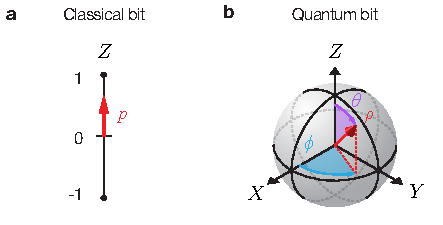
\includegraphics[scale=1.6]{mthry/BlochLineAndSphere}
\par\end{centering}
\caption[Geometric representation of the state of a classical and quantum bit]{\textbf{Geometric representation of the state of a classical and
quantum bit.} \textbf{\label{fig:Geometric-representation-of}a, }State
of a classical bit system represented as the one-dimensional probability
vector $p$ on the line segment Z between $-1$ and $1$ (see Eq.~(\ref{eq:ExpecL1})
for the definition of Z). \textbf{b, }State of quantum bit (qubit)
represented as the three-dimensional Bloch vector.  Unlike the classical
bit, the qubit has three observables (X, Y, and Z), which do not commute.
The quantum state of the qubit, $\rho$, is bounded by the unit sphere.
The surface of the sphere contains all pure states, which can be parametrized
by the angles $\phi$ and $\theta$. }
\end{figure}


\paragraph{\emph{Probabilistic bit system with perfect measurements.}}

For concreteness, consider a coin that is prepared probabilistically,
such as by a coin toss. Following the toss, an observer can perform
a measurement of the coin variable $S$, which yields a measurement
result. Formally, we should distinguish the measurement result obtained
by the observer from the actual value of the system property $S$.
For completeness, let's denote the variable of the \emph{measurement}
\emph{result} of $S$ as $m_{S}$. By analogy with $S$, we could
assign $m_{S}=-1$ and $m_{S}=1$ to results that corresponds to heads
and tails, respectively. The distinction between the measurement result
$m_{S}$ and system variable $S$ is crucial for imperfect and quantum
measurements. However, for simplicity, let us first proceed by assuming
perfect, classical measurements where there is no confusion between
$S$ and $m_{S}$, i.e, $m_{S}=S$. In this case, $m_{S}$ is redundant,
and for the following discussion there is no need to insist on the
distinction.

\emph{State of the system — a probability distribution.} To describe
the expected outcome of a measurement on the system, we introduce
the concept of the system \emph{state}.\footnote{For the following discussion, it suffices to adopt the point of view
that the state of the system represents \emph{subjective }knowledge
of the observer regarding the system. } The state describes the probability of a configuration to be the
system state. In other words, mathematically, the state is a probability
distribution over all possible system configurations, which form a
space known as the\emph{ configuration space}, denoted $\mathbb{S}$;
for the bit, $\mathbb{S}\equiv\left\{ S=1,S=-1\right\} $. The probability
for the coin be in the tails configuration, $S=1$, is then written
as $\Pr{S=1}$. More generally, the probability that the variable
$S$ of the system will have the value $s$ is $\Pr{S=s}$; for a
bit, $s\in\left\{ 1,-1\right\} $.\footnote{In this section, we employ the convention that capital letters denote
variables (typically, random ones) and lower case letters denote values.} This description of the classical system in terms of a probability
distribution, $\Pr{S=s}$, is analogous to the density matrix description
of a quantum system.\footnote{However, note that, as a probability, $\Pr{S=s}$ is a real and positive
number between 0 and 1.} Motivated by the analogy, we express the state of the coin bit as
a vector of probabilities, 
\begin{equation}
\vec{S}\equiv\begin{pmatrix}\Pr{S=1}\\
\Pr{S=-1}
\end{pmatrix}\,.\label{eq:SforBit}
\end{equation}
Keeping in mind the constraint that a measurement always yields a
result, one observes that the sum of the probabilities must be one.
Mathematically, the state vector $L^{1}$ norm is constrained, $\left|\vec{S}\right|_{\mathrm{L1}}=\sum_{s}\Pr{S=s}=1$,
where $\left|\cdot\right|_{\mathrm{L1}}$ denotes the $L^{1}$ norm.
This property is analogous to the unit-trace property of the density
matrix of a quantum state. Using this constrain, the state of the
coin, Eq.~(\ref{eq:SforBit}), can be simplified to a single information
parameter $p$, which denotes the bias of the coin,

\begin{equation}
\vec{S}=\begin{pmatrix}\frac{1+p}{2}\\
\frac{1-p}{2}
\end{pmatrix},\label{eq:BitBloch}
\end{equation}
The bias parameter $p$ is a number between $-1$ and 1,\footnote{Mathematically, $p$ is a number in the convex hull defined by $\mathbb{S}$.}
and, since it specifies the system state, is a quantity of central
importance. It can be viewed as the classical analog of the Bloch
vector of a quantum bit. In a sense, it represents a kind of one-dimensional
probability vector, which constitutes a geometric representation of
the system state; see Fig.~\ref{fig:Geometric-representation-of}a.

\paragraph{Operations on the system. }

An operation on the system results in a change of its configuration.
For the example of a coin, there are only two possible operations:
i) the coin is flipped (the logical negation operation, \emph{not})
or ii) the coin is left as is (the \emph{identity} operation). Working
within the framework of an ensemble of systems, an operation (one
that is applied to all systems in the ensemble) results in a change
of the state of the system that can be described by a linear map.
The state of the system ensemble after the operation, denoted $S'$,
can then be written as $\vec{S}'=U\vec{S}$, where the linear map
is represented by a configuration-transition matrix, denoted $U$.
For the coin, the two possible operations, the \emph{identity} and
\emph{not,} take the following forms
\begin{equation}
I\equiv\begin{pmatrix}1 & 0\\
0 & 1
\end{pmatrix}\text{\ and\ }\sigma_{x}\equiv\begin{pmatrix}0 & 1\\
1 & 0
\end{pmatrix}\,,\label{eq:IandSigmaX}
\end{equation}
respectively. The bit-flip Pauli matrix is denoted $\sigma_{x}$.


\paragraph{Perfect classical measurement of a system ensemble.}

Consider the long-run average value a series of repeated measurements
of the coin variable $S$, for the example of randomly prepared coins.
The expected mean value of $S$ is the weighted average of the results,
defined as
\begin{equation}
\E S\equiv\sum_{s}s\Pr{S=s}\,,\label{eq:EofS}
\end{equation}
where $\E{\cdot}$ represents ``expectation value of'' and the sum
is taken over all possible values $s$ of $S$. In matrix form, recalling
Eq.~(\ref{eq:BitBloch}), Eq.~(\ref{eq:EofS}) simplifies to

\begin{equation}
\E S=\left|\sigma_{Z}\vec{S}\right|_{\mathrm{L1}}=p\,,\label{eq:ExpecL1}
\end{equation}
where $p$ is non-negative and we have introduced the measurement
operator $\sigma_{Z}$, associated with the variable $S$ and given
by the Pauli matrix

\begin{equation}
\sigma_{Z}\equiv\begin{pmatrix}1 & 0\\
0 & -1
\end{pmatrix}\,.\label{eq:SigmaZ-CM}
\end{equation}
The matrix formulation given by Eq.~(\ref{eq:ExpecL1}) for the expectation
value of a classical measurement bears marked resemblance to that
employed with quantum systems. For a measurement on a quantum bit,
the expectation value of the $Z$ component of its spin is given by
$\Tr{\hat{\sigma}_{z}\rho}$, where $\rho$ is the qubit density matrix,
$\hat{\sigma}_{z}$ is the Pauli Z operator, represented by the matrix
given in Eq.~(\ref{eq:SigmaZ-CM}), and $\Tr{\cdot}$ denotes the
trace function. 

\begin{table}
\begin{centering}
\renewcommand*\arraystretch{1.5}
\begin{tabular}{l|c|>{\raggedright}p{0.5\columnwidth}}
\textbf{Concept} & \textbf{Symbols} & \textbf{Definition / Description}\tabularnewline
\hline 
\hline 
\multicolumn{3}{c}{\textbf{\rule{0pt}{5ex}Basic concepts}}\tabularnewline
\hline 
variable & $S$,$E$ & Describes intrinsic property of system, has definite value independent
of measurement apparatus\tabularnewline
\hline 
variable value & $s,e$ & Specific value that a variable can take\tabularnewline
\hline 
probability & $\Pr{S=s}$ & Probability that variable $S$ has value $s$\tabularnewline
\hline 
configuration & $\left\{ S\right\} $,$\left\{ E\right\} $,$\left\{ S,E\right\} $ & Set of all system variables\tabularnewline
\hline 
configuration space & $\mathbb{S}$,$\mathbb{E}$,$\mathbb{J}$ & Set of all possible system configurations\tabularnewline
\hline 
state  & $\vec{S},\vec{E},\vec{J}$ & Probability distribution on the configuration space, represented as
a vector\tabularnewline
\hline 
expectation value & $\E S$ & Expected (mean) value of repeated measurements of $S$, see Eq.~(\ref{eq:EofS})
\tabularnewline
\end{tabular}
\par\end{centering}
\caption[Basic concepts of classical measurement theory]{\textbf{Basic concepts of classical measurement theory.} }
\end{table}


\paragraph{Composite system. }

Extending the coin example, consider a composite system consisting
of two coins. The first coin is described by the variable $S$, or
in the ensemble situation, by the state $\vec{S}$, defined over the
configuration space $\mathbb{S}\equiv\left\{ S=1,S=-1\right\} $.
The second coin is similarly described by a single variable, $E$,
and a state $\vec{E}=\begin{pmatrix}\frac{1+p_{E}}{2}\\
\frac{1-p_{E}}{2}
\end{pmatrix}$, where $p_{E}$ is the coin bias. Its configuration space is $\mathbb{E}\equiv\left\{ E=1,E=-1\right\} $.
The configuration of the composite system consists of the simultaneous
specification of all variables, namely, $S$ and $E$. The set of
all possible configurations of the composite system is
\begin{align}
\mathbb{J} & =\mathbb{S}\otimes\mathbb{E}\label{eq:compsite-sys}\\
 & =\left\{ 1_{S},-1_{S}\right\} \otimes\left\{ 1_{E},-1_{E}\right\} \nonumber \\
 & =\left\{ 1_{S}1_{E},\,1_{S}-1_{E},\,-1_{S}1_{E},\,-1_{S}-1_{E}\right\} \,,\nonumber 
\end{align}
where $\otimes$ denotes the tensor product, and where, momentarily,
we have used the notation where $1_{S}$ stands for $S=1$.\footnote{So that no confusion arises, we note that the dimension of the composite
system space is not the sum but is the product of the subsystem dimensions,
i.e., $\dim\mathbb{J}=\dim\mathbb{S}\times\dim\mathbb{E}$, where
$\dim$ represents ``dimension of.''} The state of the composite system is a probability distribution over
$\mathbb{J}$, which can be represented by a 4-dimensional probability
vector, $\vec{J}$. When the two subsystems are uncorrelated, the
composite state is separable, and can be written as a simple product
of the states of the constituent subsystems, $\vec{J}=\vec{S}\otimes\vec{E}$.
However, when the subsystems are correlated, this is no longer possible.
For concreteness, consider the case where the two coins are prepared
randomly but always the same, the correlated randomness of the two
systems is described by the composite state  $\vec{J}=\left(\frac{1}{2},0,0,\frac{1}{2}\right)^{\intercal}$,
where $^{\intercal}$ denotes the transposition operation. More generally,
an operation that represents an interaction between the two coins
results in statistical correlations between them, and thus renders
the composite state inseparable. These features generally carry over
to the description of composite quantum systems, but standard statistical
correlations are replaced by entanglement. In the following subsection,
Sec.~\ref{subsec:Classical-model-of}, we explore the effect of an
interaction between the two coins.

\subsection{Classical toy model of system-environment interaction\label{subsec:Classical-model-of}}

For a more general discussion of measurements, it is necessary to
consider the interaction of the system with another, which probes
it and is often referred to as the \emph{environment}. In this subsection,
we consider the minimal limit of this model, where both the system
and environment are bits. Further, to introduce only the essentials
for now, we consider only the effect of a single interaction between
the classical system and environment, and discuss the effect of the
interaction on the system transfer of information. In the following
subsection, Sec.~\ref{subsec:Quantum-model-of}, we consider the
analogous quantum case, consisting of the interaction between a system
and environment, each of which is quantum bit. In Sec.~\ref{sec:Introductory-example:-qubit},
we generalize the toy model to the time-continuous homodyne monitoring
of a quantum bit. 

\begin{figure}
\begin{centering}
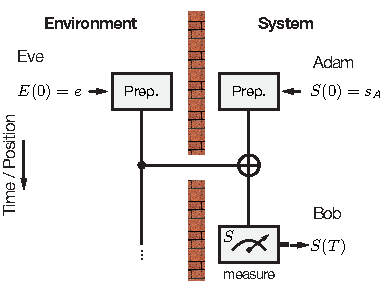
\includegraphics[scale=1.5]{mthry/SamAndEve}
\par\end{centering}
\caption[Classical toy model of the interaction between the system and environment]{\textbf{\label{fig:Reversibility-of-classical}Classical} \textbf{toy
model of the interaction between the system and environment.} Circuit
of the interaction between the system, with agents Adam and Bob, and
the environment, with agent Eve. Vertical lines depict the bits of
the system and environment, initially prepared by Adam and Eve in
the states $S\left(0\right)=s_{A}$ and $E\left(T\right)=e$, respectively.
The two bits interact via a controlled-NOT (cNOT) gate. Bob measures
the system at time $T$, obtaining the value $S\left(T\right)$. Brick
wall depicts the lack of communication between the agents of the system
and environment. }
\end{figure}


\paragraph{Classical toy model. }

Continuing with the example of two coins, we label one as the ``system''
and the other as the ``environment.'' For definitiveness, consider
the case where the system coin belongs to Adam, who aims to employ
it to communicate with Bob. To achieve this, at time $t=0$, Adam
prepares his coin in the configuration $S\left(0\right)=s_{A}$, where
$s_{A}$ is the bit value Adam hopes to communicate. He sends the
coin flying to Bob, who receives it at time $T$, and measures it
to obtain the value of $S\left(T\right)$. If the coin flies undisturbed,
$S\left(T\right)=S\left(0\right)$, and Bob faithfully receives Adam's
bit. 

However, during its flight, the coin unavoidably interacts with a
second flying coin, which belongs to an agent, Eve, who, at time $t=0$,
has prepared her coin in the configuration $E\left(0\right)=e$, where
$E$ is the variable describing her coin, and which is unknown to
Adam and Bob. For concreteness, suppose the interaction between the
two coins is described by the controlled-NOT (cNOT) gate, 
\begin{equation}
\mathrm{cNOT}\equiv I\otimes\begin{pmatrix}1 & 0\\
0 & 0
\end{pmatrix}+\sigma_{x}\otimes\begin{pmatrix}0 & 0\\
0 & 1
\end{pmatrix}=\begin{pmatrix}1 & 0 & 0 & 0\\
0 & 0 & 0 & 1\\
0 & 0 & 1 & 0\\
0 & 1 & 0 & 0
\end{pmatrix}\,,\label{eq:cNOT}
\end{equation}
where I and $\sigma_{x}$ are defined according to Eq.~(\ref{eq:IandSigmaX}).
Matrices associated with operations on the system (resp: environment)
are placed to the left (resp: right) of the tensor product. Given
that Adam and Bob lack knowledge of Eve's bit value, $e$, but are
aware of the interaction, to what degree can they communicate, i.e.,
what is the effect of the interaction on the value, $S\left(T\right)$,
measured by Bob?  More importantly, what action can Bob undertake
to undo the effect of the interaction, so as to obtain Adam's bit,
$S\left(T\right)=S\left(0\right)$? 

\paragraph{Evolution of the state, and Bob's information gain. }

Employing the formalism developed in Section~\ref{subsec:Classical-measurement-theory-basic-concept},
the initial state of the composite system, consisting of the two coins,
is described by the state vector $\vec{J}\left(0\right)=\vec{S}\left(0\right)\otimes\vec{E}\left(0\right),$
where the initial states of the system and environment are $\vec{S}\left(0\right)=\begin{pmatrix}\frac{1+s_{A}}{2}\\
\frac{1-s_{A}}{2}
\end{pmatrix}$ and $\vec{E}\left(0\right)=\begin{pmatrix}\frac{1+p_{E}}{2}\\
\frac{1-p_{E}}{2}
\end{pmatrix},$ respectively. The variable $p_{E}$ denotes the bias of Eve's coin,
see Eq.~(\ref{eq:BitBloch}). Following the interaction, the composite
system state is given by $\vec{J}\left(T\right)=\mathrm{cNOT\,}\vec{J}\left(0\right)$.
The expected mean value of Bob's measurement of $S\left(T\right)$,
represented by the matrix $I\otimes\sigma_{z}$, is given by, recalling
Eq.~(\ref{eq:ExpecL1}),
\begin{equation}
\E{S\left(T\right)}=\left|\left(I\otimes\sigma_{z}\right)\vec{J}\right|_{\mathrm{L1}}=p_{E}s_{A}.\label{eq:EsSamAdam}
\end{equation}
To understand Eq.~(\ref{eq:EsSamAdam}), consider three limiting
cases: i) Eve always prepares her coin facing up, $e=1$, corresponding
to a maximal coin bias, $p_{E}=1$. Since for $e=1$ the interaction
with her coin has no effect on Adam's coin, Bob faithfully receives
Adam's bit every time, $\E{S\left(T\right)}=s_{A}$. ii) Eve always
prepares her coin facing down, $e=-1$. Since her coin bias is now
$p_{E}=-1$, Bob always receives Adam's coin flipped $\E{S\left(T\right)}=-s_{A}$.
While inconvenient for Bob, by flipping each coin he receives (a deterministic
action), he could recover the bit. The effect of Eve's coin is to
change the encoding of the information, but has not resulted in its
loss. iii) Eve prepares her coin completely randomly, $p_{E}=0$.
On average, Bob receives no information from Adam, $\E{S\left(T\right)}=0$!
Eve has  randomly scrambled the encoding of the information for each
of the realizations, which, from Bob's point of view, results in the
complete loss of the initial system information encoded by Adam. More
generally, for an arbitrary coin bias $p_{E}$, the information shared
between Adam and Bob is characterized by the correlation between the
initial and final configurations of the system, which is given by
the bias of Eve's bit, $\E{S\left(T\right)S\left(0\right)}=p_{E}$,
which can be understood as the result of information transfer between
the system and environment, facilitated by the cNOT interaction, however,
where the ``information'' propagating to the system from the environment
is random noise. 

While the transfer of information between Adam and Bob is degraded
by the influence of the interaction with Eve's bit, in principle no
information has been erased, because the cNOT interaction is reversible.
For the case where $p_{E}=0$, Adams bit, $s_{A}$, is not transferred
to Bob at all; rather, it is encoded in the correlation between the
system and environment, $\E{S\left(T\right)E\left(T\right)}=\left|\left(\sigma_{z}\otimes\sigma_{z}\right)\vec{J}\right|_{\mathrm{L1}}=s_{A}$,
which is inaccessible to Adam and Bob, who only have control over
the system coin, and, hence, only access to $S$. To summarize, the
interaction between the system and a randomly prepared random environment
results in loss of information and injection of noise into the system,
as far as the system alone is concerned. Nevertheless, from the vantage
point of the composite system, no information is lost; rather, it
is transferred into correlations between the system and environment. 

\paragraph{Recovering the information.}

To recover Adam's bit, Bob requires access to Eve's physical coin
or knowledge of $e$, the specific value of her coin for \emph{each}
realization. First, consider the latter case, where Bob learns $e$.
Recalling that $\mathrm{cNOT}^{2}=I\otimes I$, before Bob performs
a measurement, he can undo the interaction effect by preparing an
ancillary, third, coin with the value $e$, by employing it to perform
a second cNOT operation on his coin, thus reversing the first. Applied
to each realization, this procedure results in faithful communication,
$\E{S\left(T\right)S\left(0\right)}=1$. Notably, Bob can also reverse
the interaction effect\emph{ after} performing his measurement by
essentially applying the second cNOT operation virtually, i.e., when
$e=1$, $s_{A}=s_{B}$, while otherwise, $s_{A}=-s_{B}$. We remark
that any operations performed by Eve on her coin after the system-environment
interaction have no consequences for Bob. To summarize, the examples
highlights three distinct aspects regarding the recovery of information
in the classical setting:
\begin{enumerate}
\item Eve's physical system was not required, only information about its
initial configuration, $E\left(0\right)=e$.
\item The effect of the interaction can be reversed \emph{before} or \emph{after}
Bob's measurement. 
\item Operations on Eve's coin subsequent to the interaction have no consequences.
\end{enumerate}
All three of these features break down in the quantum setting, as
discussed in the following subsection. 

\subsection{Quantum toy model\label{subsec:Quantum-model-of}}

Rather than communicating with classical bits (coins), consider the
situation where Adam and Bob communicate with quantum bits (qubits),
and Eve too employs a qubit. Before proceeding, we briefly review
the basic qubit concepts.

\paragraph{Quantum bit. }

While the fundamental concept of classical information is the bit,
which represents the minimal classical system, the fundamental concept
of quantum information is the \emph{quantum bit}, or \emph{qubit}
for short, which represents the minimal physical quantum system. A
qubit has two basis states, $\ket{+z}$ and $\ket{-z}$. A pure state
of the qubit  is described by the state $\ket{\psi}=\cos\left(\frac{\theta}{2}\right)\ket{+z}+e^{i\phi}\sin\left(\frac{\theta}{2}\right)\ket{+z}$,
where the angles $\theta$ and $\phi$, which fall in the range $0\leq\theta\leq\pi$
and $0\leq\phi\leq2\pi$, define a point on the unit sphere, known
as the \emph{Bloch sphere}, see Fig.~\ref{fig:Geometric-representation-of}b.
 More generally, a statistical ensemble of pure states, a \emph{mixed}
qubit state is described by the density matrix 
\begin{equation}
\rho=\frac{1}{2}\left(\hat{I}+X\hat{\sigma}_{x}+Y\hat{\sigma}_{y}+Z\hat{\sigma}_{z}\right)\,,
\end{equation}
where $X$, $Y$, $Z$ are real numbers parameterizing the state,
given by the averages of the Pauli operators, $X\equiv\Tr{\hat{\sigma}_{x}\rho}$,
\emph{et cetera}, where $\Tr{\cdot}$ denotes the trace operation.
The matrix representation of the identity, $\hat{I}$, and Pauli $\hat{\sigma}_{x}$
and $\hat{\sigma}_{z}$ operators is given in Eqs.~(\ref{eq:IandSigmaX})
and (\ref{eq:SigmaZ-CM}), while that of Pauli operator Y is $\hat{\sigma}_{y}=\begin{pmatrix}0 & -i\\
i & 0
\end{pmatrix}$, where $i$ is the unit imaginary. The Bloch vector, $\left(X,Y,Z\right)^{\intercal}$,
provides an important geometrical representation of the state of the
qubit, and as discussed in Sec.~\ref{subsec:Classical-measurement-theory-basic-concept}
is the analog of the coin bias $p$. For a pure state, the Bloch vector
extends to the surface of the Bloch sphere, while for mixed states,
it lies in the interior. Notably, it admits the spherical parameterization:
\begin{align}
X & =r\sin\left(\theta\right)\cos\left(\phi\right)\,,\nonumber \\
Y & =r\sin\left(\theta\right)\sin\left(\phi\right)\,,\nonumber \\
Z & =r\cos\left(\theta\right)\,,\label{eq:XYZBLoch}
\end{align}
where the angles $\theta$ and $\phi$ are defined as for pure states
and $r$ is the length of the Bloch vector, a number between 0 and
1. Notably, in the Bloch representation, mutually orthogonal state
vectors are \emph{not} represented by orthogonal Bloch vectors, but
rather, by opposite Bloch vectors, which specify antipodal points
on the sphere. 

\paragraph{Quantum toy model. }

Returning to the toy model example of the interaction between two
systems (recall Fig.~\ref{fig:Reversibility-of-classical}, which
depicts the analogous classical model), we consider the case where
at time $t=0$ Adam prepares his qubit in the pure state $\ket{\psi\left(0\right)}$,
with corresponding Bloch vector components $X\left(0\right)$, $Y\left(0\right)$,
and $Z\left(0\right)$, while Eve prepares her qubit in the pure state
$\ket{+x}$, where $\ket{+x}=\frac{1}{\sqrt{2}}\left(\ket{+z}+\ket{+z}\right)$.
Unlike in the classical toy model, Adam has a choice regarding the
encoding of his information — the orientation of the Bloch vector,
which has no classical analog. Both qubits are sent flying. A controlled-NOT
interaction occurs, described by the operator $\mathrm{cNOT}=\hat{I}\otimes\kb{+z}{+z}+\hat{\sigma}_{x}\otimes\kb{-z}{-z}$,
where operators on the left (resp., right) of the tensor product,
denoted $\otimes$, act on the system (resp., environment). Notably,
the matrix representation of the cNOT operator is the same that of
the classical cNOT gate, given in Eq.~(\ref{eq:cNOT}). After the
interaction Bob receives the system qubit, at time $T$. 

\paragraph{Effect of the interaction before the measurement. }

Before the measurement, the pure state of the composite system, $\ket{\Psi\left(T\right)}=\mathrm{cNOT}\left(\ket{\psi\left(0\right)}\ket{+x}\right)$,
is, in general, inseparable — it cannot be written as a simple product
of states of its component systems. On a mathematical level, this
result is the same as that for the classical model; however, the interpretation
and consequences are markedly distinct. Classically, the inseparability
represented statistical correlations between \emph{definite} configurations
of the system and environment. For the quantum model, the inseparability
represents entanglement between the system and environment — the system
cannot be fully described without considering the environment. Generally,
measurements of the entangled system are correlated with those of
the environment, and the system alone cannot be represented by a pure
state. The consequences of the system-environment entanglement are
at the heart of quantum measurement theory. 

Consider the reduced density matrix of the system qubit, found by
taking the partial trace over the environment, denoted $\mathrm{Tr}_{E}\left[\cdot\right]$,
\begin{equation}
\rho_{S}\left(T\right)=\mathrm{Tr}_{E}\left[\ketbra{\Psi\left(T\right)}{\Psi\left(T\right)}\right]=\frac{1}{2}\begin{pmatrix}1 & X\left(0\right)\\
X\left(0\right) & 1
\end{pmatrix}\,.\label{eq:rho_s-env-q}
\end{equation}
Evidently, entanglement in the composite state, the result of the
interaction between the system and environment results in the loss
of information from the point of view of the system. Specifically,
the $Y$ and $Z$ Bloch components prepared by Adam, $Y\left(0\right)$
and $Z\left(0\right)$, are absent in $\rho_{S}\left(T\right)$, despite
the deterministic preparation of the ancilla in a\emph{ pure} state
$\ket{+x}$. However, if Adam chose to encode his information along
the X component of the Bloch vector, it would propagate to Bob undisturbed
by the interaction with the environment, and Bob could receive it
by measuring $X$. It is the $X$ component that is preserved due
to the choice of the interaction and initial pure state of the environment.
Analogously to the classical case, no information is truly lost, but
rather, when viewed in the broader context of the composite system,
Adam's initial $Y$ and $Z$ qubit components are encoded in the YZ,
$\left\langle YZ\right\rangle \equiv\Tr{\left(\hat{\sigma}_{y}\otimes\hat{\sigma}_{z}\right)\rho}=Y\left(0\right)$,
and ZZ, $\left\langle ZZ\right\rangle \equiv\Tr{\left(\hat{\sigma}_{z}\otimes\hat{\sigma}_{z}\right)\rho}=Z\left(0\right)$,
correlations between the system and environment, respectively.


\paragraph{Recovering information before the measurement. }

In the classical case, by learning the initial configuration of the
environment, $E\left(0\right)=e$, Bob could undo the effect of the
system-environment interaction and could recover the state sent by
Adam before performing the measurement. In the quantum case, this
is not possible. Even though Bob can know the initial state, $\ket{+x}$,
of the environment and can clone it, by preparing a third ancilla
qubit in the state $\ket{+x}$, he cannot use this ancilla to perform
a second cNOT operation on the system so as to reverse (recall that
$\mathrm{cNOT}^{2}=\hat{I}$) the cNOT performed by the environment
qubit. This is a profound consequence of the entanglement between
the system and environment, and has no classical analog. The only
way to reverse the interaction is to use the physical qubit of the
environment to perform the second cNOT operation — \emph{no} clone
will suffice. 

\paragraph{Projective (von Neumann) measurement.\label{par:Projective-(von-Neumann)}}

For a classical system described by a state of maximal knowledge,
the result of any measurement can be determined with certainty. However,
for a quantum system described by a state of maximal knowledge, a
pure state, the result of a measurement is \emph{not}, in general,
determined. For definitiveness, consider the description of a perfect
projective (von Neumann) measurement performed by Bob on the $Z$
component of his qubit spin, with the associated  operator (\emph{observable})
$\hat{\sigma}_{z}$.  The measurement is described by the spectral
decomposition of the observable, $\hat{\sigma}_{z}=\sum_{r}r\hat{\pi}_{r}=\hat{\pi}_{1}-\hat{\pi}_{-1}$,
where $r$ is an eigenvalue, $r=1$ or $r=-1$, to which corresponds
a measurement result, and $\hat{\pi}_{r}$ is the projection operator
onto the eigenstate associated with $r$, $\hat{\pi}_{1}=\kb{+z}{+z}$
and $\hat{\pi}_{-1}=\kb{+z}{+z}$. The probability of obtaining an
outcome corresponding to the eigenvalue $r$ is
\begin{equation}
\wp_{r}=\Tr{\hat{\pi}_{r}\rho}\,.\label{eq:ProbOfprojMsr}
\end{equation}
According to the projection postulate of quantum mechanics,\footnote{Curiously, the modern formulation of the projection postulate is not
precisely that of von Neumann \citep{VonNeumann1932}, but contains
a correction due to Lüders \citep{Luders1951}. } the measurement leads to the projection (or ``collapse'')\footnote{W. Heisenberg introduced the idea of wavefunction collapse in 1927
\citep{Heisenberg1927}.} of the system state into an eigenstate of the measurement operator.
Immediately after the measurement, conditioned on the result $r$,
the state of the system is 
\begin{equation}
\rho_{r}=\frac{\hat{\pi}_{r}\rho\hat{\pi}_{r}}{\wp_{r}}\,.\label{eq:projectionPostulate}
\end{equation}
The evolution due to Eq.~(\ref{eq:projectionPostulate}) is markedly
non-linear in the state density, which appears in the denominator,
and represents a radical departure from the linear evolution encountered
with Schrödinger’s equation. Further, while a perfect measurement
of a classical system does \emph{not} alter its state, a perfect measurement
of a quantum system, in general, \emph{does} alter its state. This
non-linear disturbance has profound consequences.

Suppose, at time $T$, Bob performs a $Z$ measurement of his qubit
and obtains the result $r=1$, with probability, recalling Eqs.~(\ref{eq:rho_s-env-q})
and~(\ref{eq:ProbOfprojMsr}), $\wp_{1}=\Tr{\hat{\pi}_{1}\rho_{S}\left(T\right)}=\frac{1}{2}$.
Note that $\wp_{1}$ is independent of $X\left(0\right)$, $Y\left(0\right)$,
and $Z\left(0\right)$. The system state after the measurement is
$\rho_{1}=\hat{\pi}_{1}\rho_{S}\left(T\right)\hat{\pi}_{1}/\Tr{\rho_{S}\left(T\right)\hat{\pi}_{1}}=\begin{pmatrix}1 & 0\\
0 & 0
\end{pmatrix}$, corresponding to the pure state $\ket{+z}$. Notably, the potentially
recoverable information encoded by Adam, $X(0)$, is irreversibly
lost. From the point of view of the composite system, described by
the state $\ket{\Psi\left(T\right)}$, the measurement has projected
the state onto the measurement basis, according to the effect of the
projector $\hat{\pi}_{1}\otimes\hat{I}$. The state of the composite
system after the measurement, $\ket{+z}\ket{\psi\left(0\right)}$,
is pure and separable, i.e., the measurement has disentangled the
system and environment. In this toy model (and for this particular
measurement outcome), it just so happens that Adam's state is completely
teleported to Eve's qubit, a form of information transfer between
the two systems. To understand the situation a bit better, consider
the alternative, where $r=-1$, with the associated projector $\hat{\pi}_{-1}\otimes\hat{I}$.
The conditional state of the system after the measurement is again
obtained by employing Eq.~(\ref{eq:projectionPostulate}), yielding
$\ket{+z}\ket{\psi'}$ for the composite system, where the state $\ket{\psi'}$
has the same Bloch vector as Adam's initial state $\ket{\psi\left(0\right)}$
but with the $Y$ and $Z$ components flipped. This example illustrates
the more general feature that a measurement on either the system or
environment disentangles the two, resulting in a perfect correlation
between the measurement on one and the state of the other. Further,
it tends to lead to a transfer of information between the two subsystems.
We explore the profound consequences of these features in the following
section.


\section{Continuous quantum measurements: introduction to quantum trajectories
and stochastic calculus \label{sec:Introductory-example:-qubit} }

In this section, we consider a heuristic microscopic model of continuous
quantum measurements, which, although simple, contains sufficient
generality to introduce the principal ideas. Specifically, we model
the homodyne measurement of a qubit by a sequence of interactions
with a chain of identically prepared ancilla qubits.  A chain of
ancillary systems modeling the environment is known as a von Neumann
chain \citep{VonNeumann1932}. While the evolution due to the interaction
with each ancilla is unitary, ``deterministic,'' the addition of
a projective (von Neumann) measurement of each ancilla subsequent
to its interaction with the system results in the stochastic evolution
of the quantum state of the system — known as a\emph{ quantum trajectory}
\citep{Carmichael1993}. Due to the correlation between the state
of a measured ancilla and the resulting  state of the system, the
measurement results allow faithful tracking of the state trajectory
\citep{belavkin1987non,Carmichael1993,Gardiner1992-original-traj,Dalibard1992-original-traj,Korotkov1999-original-traj}.
After introducing the time-discrete version of the model, we take
its continuum limit, which allows us to introduce the fundamental
concepts of stochastic calculus. Specifically, we focus on introducing
the Wiener noise process and obtaining the stochastic differential
equations (SDEs) that describe the homodyne monitoring of the qubit.
Most of the results derived in this section carry over with little
modification to the following section, Sec.~\ref{sec:Quantum-trajectory-theory},
which establishes the general formulation of quantum measurement theory.
Time-discrete chain models have been discussed in Refs.~\citet{Caves1987-time-discrete,Attal2006,Tilloy2015,Korotkov2016-qm-bayes,Bardet2017}.

 

\subsection{Time-discrete model with flying spins}

\begin{figure}
\begin{centering}
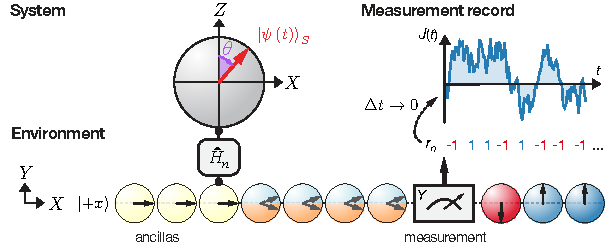
\includegraphics[scale=1.4]{mthry/SpinBathModelFigure}
\par\end{centering}
\caption[Homodyne monitoring of a quantum bit: time-discrete model]{\textbf{\label{fig:Ch2:SpinBathModel1}Homodyne monitoring of a quantum
bit: time-discrete model.} The qubit, whose Bloch vector lies in the
XZ plane, sequentially interacts with a chain of ancilla qubits, which
model the environment. At the beginning of each timestep, at time
$t$, the system is in a pure state, $\ket{\psi\left(t\right)}_{S}$.
During the $n$-th timestep, of length $\Delta t$, the qubit interacts,
subject to the Hamiltonian $\hat{H}_{n}$, with the $n$-th ancilla,
prepared in $\ket{+x}$, whereafter, the Y component of its spin is
projectively measured. The result of the measurement, $r_{n}$, which
is either -1 or 1, is recorded and accumulated; in the continuum limit,
$\Delta t\rightarrow0$, it leads to the homodyne signal $J\left(t\right)$,
a time-continuous stochastic (Weiner) process.}
\end{figure}

Time is discretized in small but finite bins of length $\Delta t$
labeled by the integer $n$, i.e.,~$t=n\Delta t$. During each timestep,
a single spin of the environment, referred to as the \emph{ancilla},
interacts with the system for time $\Delta t$, see Fig.~\ref{fig:Ch2:SpinBathModel1}.
For simplicity, assume each spin is identically prepared in the state
$\ket{+x}$. We employ the convention that the states $\ket{\pm x}$,
$\ket{\pm y}$, and $\ket{\pm z}$ denote eigenstates of the Pauli
X, Y, and Z operators, respectively. The interaction between the $n$-th
ancilla and the system is described by the Hamiltonian 
\begin{equation}
\hat{H}_{n}\equiv-\frac{\hbar\lambda}{2}\hat{\sigma}_{z}^{S}\otimes\hat{\sigma}_{z}^{\left(n\right)}\,,
\end{equation}
where $\lambda$ is the strength of the interaction, $\hbar$ is Plank's
constant, and $\hat{\sigma}_{z}^{S}$ and $\hat{\sigma}_{z}^{\left(n\right)}$
denote the Pauli Z operators of the system and ancilla, respectively.
For the time being, we assume that $\hat{H}_{n}$ is the only generator
of system evolution, and the system Hamiltonian is zero, $\hat{H}_{S}=0$.
Following the interaction, the ancilla is measured by a detector that
performs a projective measurement of the ancilla spin  Y component,
which yields the measurement result $r_{n}=-1$ or $r_{n}=1$. The
observer operating the measurement apparatus keeps track of the sum
total of the measurement results, the measurement signal: $J_{t}\equiv\sqrt{\Delta t}\sum_{n'=0}^{n}r_{n'}$. 

Note two assumptions  regarding the measurement: i) the ancilla qubits
are undisturbed during their flight from the system to the measurement
apparatus, and ii) the measurement apparatus performs a perfect measurement,
and does not add technical noise. These assumptions ensure no information
is lost in the measurement, nor spurious noise is added by it; i.e.,
the observer has perfect access to all information there is to know
in the environment, and is hence referred to as an \emph{omniscient}
\emph{observer}. 

\subparagraph{Evolution of the composite system. }

For simplicity, assume the state of the system at time $t$ is pure
and its Bloch vector lies in the XZ plane; i.e., it is described by
a single angle $\theta\left(t\right)$, 
\begin{align}
\ket{\psi\left(t\right)}_{S} & =\cos\left(\frac{\theta\left(t\right)}{2}\right)\ket{+z}_{S}+\sin\left(\frac{\theta\left(t\right)}{2}\right)\ket{-z}_{S}=\begin{pmatrix}\cos\left(\frac{\theta\left(t\right)}{2}\right)\\
\sin\left(\frac{\theta\left(t\right)}{2}\right)
\end{pmatrix}\,.\label{eq:SpinBath:sysState}
\end{align}
The state of the composite system at time $t$, consisting of the
$n$-th ancilla and the system qubit, is $\ket{\Psi\left(t\right)}=\ket{\psi\left(t\right)}_{S}\otimes\ket{+x}_{n}$,
and for duration $\Delta t$ evolves subject to the Hamiltonian $\hat{H}_{n}$.
The total evolution is given by the propagator $\hat{U}\left(t,t+\Delta t\right)=\exp\left(-i\hat{H}_{n}\Delta t/\hbar\right)$,
and the composite-system state after the interaction is 
\begin{equation}
\ket{\Psi\left(t+\Delta t\right)}=\hat{U}\left(t,t+\Delta t\right)\ket{\Psi\left(t\right)}\,,
\end{equation}
Anticipating the ancilla Y measurement, we express $\ket{\Psi\left(t+\Delta t\right)}$
in terms of the measurement operator eigenstates. The measurement
operator on the ancilla alone is the Pauli Y operator, $\hat{\sigma}_{y}^{\left(n\right)}$,
with eigenstates $\ket{-y}_{n}$ and $\ket{+y}_{n}$, in terms of
which, 
\begin{equation}
\ket{\Psi\left(t+\dt\right)}=\ket{\tilde{\psi}_{-1}\left(t+\Delta t\right)}_{S}\otimes\ket{-y}_{n}+\ket{\tilde{\psi}_{+1}\left(t+\Delta t\right)}_{S}\otimes\ket{+y}_{n}\,,\label{eq:PsiQubitEnvSpin}
\end{equation}
where the parameter $\epsilon\equiv\lambda\Delta t$ characterizes
the measurement strength and the un-normalized\footnote{By convention, a tilde will indicate an unnormalized state, with a
norm less than one.} system states $\ket{\tilde{\psi}_{\pm1}\left(t+\Delta t\right)}_{S}$
are
\begin{equation}
\ket{\tilde{\psi}_{\pm1}\left(t+\Delta t\right)}_{S}\equiv\begin{pmatrix}\cos\left(\frac{\theta\left(t\right)}{2}\right)\cos\left(\frac{\pi/2\pm\epsilon}{2}\right)\\
\sin\left(\frac{\theta\left(t\right)}{2}\right)\sin\left(\frac{\pi/2\pm\epsilon}{2}\right)
\end{pmatrix}_{S}\,.\label{eq:SpinBath:psiTilde}
\end{equation}
The state of the composite system following the interaction, Eq.~(\ref{eq:PsiQubitEnvSpin}),
is not separable. The interaction has entangled the system and environment,
as discussed of Sec.~\ref{subsec:Quantum-model-of}.

\paragraph{Projective (von Neumann) measurement of the ancilla. }

The action of the measurement apparatus on the composite system is
described, recalling the discussion on Pg.~\pageref{par:Projective-(von-Neumann)},
by decomposing the measurement operator $\hat{Y}_{n}=\hat{I}\otimes\hat{\sigma}_{y}$
in terms of its  eigenstate projectors, $\hat{\pi}_{\pm}\equiv\hat{I}_{S}\otimes\left(\kb{\pm y}{\pm y}\right)_{n}$;
note, $\hat{Y}=\hat{\pi}_{+}-\hat{\pi}_{-}$. According to the von~Neumann
postulate, the projectors yield the probability for obtaining the
results $r_{n}=-1$ and $r_{n}=1$ from the measurement, 
\begin{align}
\wp_{r}\left(t\right) & =\bra{\Psi\left(t+\Delta t\right)}\hat{\pi}_{r}\ket{\Psi\left(t+\Delta t\right)}\nonumber \\
 & =\braket{\tilde{\psi}_{r}\left(t+\Delta t\right)}{\tilde{\psi}_{r}\left(t+\Delta t\right)}\nonumber \\
 & =\frac{1}{2}\left(1-r_{n}\sin\left(\epsilon\right)\cos\left(\theta\left(t\right)\right)\right)\,,\label{eq:PflyingSpinPM1}
\end{align}
as well as the state of the composite system immediately after the
measurement, conditioned on the result $r_{n}$, 
\begin{equation}
\ket{\Psi_{r}\left(t+\Delta t\right)}=\ket{\tilde{\psi}_{r}\left(t+\Delta t\right)}_{S}\ket{y:=r}_{n}/\sqrt{\wp_{r}\left(t\right)},\label{eq:Psir_afterMsr}
\end{equation}
where $\ket{y:=r}_{n}$ denotes ancilla state $\ket{+y}_{n}$ (resp.,
$\ket{-y}_{n}$) for $r=1$ (resp., $r=-1$). The measurement has
transformed the entanglement between the system and environment, evident
in the non-separable state $\ket{\Psi\left(t+\Delta t\right)}$, Eq.~(\ref{eq:PsiQubitEnvSpin}),
into a correlation between the pure state of the system and environment
after the measurement, evident in the separable, non-entangled conditional
state $\ket{\Psi_{r}\left(t+\Delta t\right)}$, Eq.~(\ref{eq:Psir_afterMsr}).
Assuming the ancilla never interacts with the system again, it is
unnecessary to retain it in the description of the measurement; removing
it from Eq.~(\ref{eq:Psir_afterMsr}), we obtain the pure state of
the system alone at time $t+\Delta t$:
\begin{align}
\ket{\psi_{r}\left(t+\Delta t\right)}_{S} & =\frac{1}{\sqrt{\wp_{r}\left(t\right)}}\ket{\tilde{\psi}_{r}\left(t+\Delta t\right)}_{S}=\begin{pmatrix}\cos\left(\frac{\theta_{r}\left(t+\dt\right)}{2}\right)\\
\sin\left(\frac{\theta_{r}\left(t+\dt\right)}{2}\right)
\end{pmatrix}\,.\label{eq:SpinModel:postState}
\end{align}
From the point of view of the observer, the entanglement is transformed
by the measurement into a classical correlation between the result
$r_{n}$ and the final conditional state of the system, $\ket{\psi_{r}\left(t+\Delta t\right)}_{S}$.
Figure~\ref{fig:Ch2:SpinBath} summarizes the steps of the model
and the conditional state update.

\begin{figure}
\begin{centering}
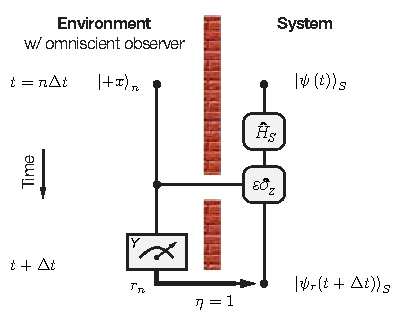
\includegraphics[scale=1.4]{mthry/SpinBathModel}
\par\end{centering}
\caption[Circuit representation of the $n$-th timestep of the quantum trajectory]{\textbf{\label{fig:Ch2:SpinBath}Circuit representation of the $n$-th
timestep of the quantum trajectory. }At time $t=n\Delta t$, the system,
described by the state $\ket{\psi\left(t\right)}_{S}$, is subjected
to the system Hamiltonian $\hat{H}_{S}$ and the interaction with
the $n$-th ancilla, characterized by the parameter $\epsilon$. Every
ancilla is prepared in $\ket{+x}$. Following the interaction, the
detector projectively measures the Y component of the ancilla spin,
yielding the result $r_{n}$, which provides the information necessary
to update the state of the system. In the case of the omniscient observer,
characterized by unit quantum measurement efficiency, $\eta=1$, at
the end of the timestep, immediately after $t+\Delta$, the system
state, $\ket{\psi_{r}\left(t+\Delta t\right)}_{S}$, conditioned on
the measurement result is pure. Contrast with Fig.~\ref{fig:Reversibility-of-classical}. }
\end{figure}


\paragraph{Solution for the conditional state update. }

To explicitly solve Eq.~(\ref{eq:SpinModel:postState}) for the updated
angle of the qubit system conditioned on the measurement result $r_{n}$,
$\theta_{r}\left(t+\Delta t\right)$, one can use Eqs.~(\ref{eq:PflyingSpinPM1})
and~(\ref{eq:SpinBath:psiTilde}), following trigonometric manipulation,
to obtain, without any approximations, an explicit relation (\citeauthor{MHD})
between the Bloch angle at the start and end of the timestep: 
\begin{equation}
\boxed{\tan\left(\frac{\theta_{r}\left(t+\Delta t\right)}{2}\right)=\tan\left(\frac{\theta\left(t\right)}{2}\right)\tan\left(\frac{\pi/2+r_{n}\epsilon}{2}\right)\,.}\label{eq:SpinBath:Ch2:tan}
\end{equation}
In the following section, Sec.~\ref{subsec:Random-walk-on}, this
seemingly non-linear equation is transformed into a linear equation
by a hyperbolic transformation of the circular angle $\theta$, and
is solved exactly. Nonetheless, for the continuum-limit discussion
in Sec.~\ref{subsec:Continuous-limit:-Wiener}, consider the solution
of Eq.~(\ref{eq:SpinBath:Ch2:tan}) in the limit of weak interactions,
$\epsilon\ll1$, to order $\epsilon$: 
\begin{equation}
\mathrm{d}\theta\left(t\right)\equiv\theta\left(t+\Delta t\right)-\theta\left(t\right)\approx\epsilon r_{n}X\left(t\right)\,,\label{eq:SPinBath:ThPM}
\end{equation}
where we have defined the Bloch angle increment, $\mathrm{d}\theta\left(t\right)$,
and $X\left(t\right)$ is the X component of the Bloch vector, $X\left(t\right)=\sin\left(\theta\left(t\right)\right)$. 

\paragraph{Interpretation and remarks. }

The system measurement dynamics are described in entirety by Eqs.~(\ref{eq:PflyingSpinPM1}),~(\ref{eq:SpinModel:postState}),
and~(\ref{eq:SPinBath:ThPM}). To make the discussion more concrete,
consider the particular case where the system and ancilla do not interact,
$\epsilon=0$. The measurement results are completely random, $\wp_{r}=\frac{1}{2}$,
uncorrelated with the system; similarly, the system state is independent
of the measurement results, $r_{n}$; in fact, there is no state evolution,
$\mathrm{d}\theta\left(t\right)=0$. Consider the more interesting
case of weak interactions, $\epsilon\ll1$. Measurement results are
correlated with the Z component of the system Bloch vector, $\wp_{r}=\frac{1}{2}\left(1-\epsilon r_{n}Z\left(t\right)\right)$,
where $Z\left(t\right)=\cos\left(\theta\left(t\right)\right)$. Nonetheless,
 due to $\epsilon\ll1$, the two measurement results still occur with
nearly equal probability, and the record consists of random noise,
but with a slight bias that correlates it with $Z$. Thus, the value
of $Z$ can be obtained from the instantaneous average of the measurement
results, $\E{r_{n}}=-\epsilon Z$. In time, from the point of view
of the observer, a long sequence of measurements gradually results
in the complete measurement of $Z$, obtained from the noisy measurement
record. A peculiar feature of the weak interaction regime, $\epsilon\ll1$,
is that amplitude of the noise is essentially constant for all measurement
strengths, its variance is $\mathrm{Var}\left[r_{n}\right]=1-\left(\epsilon Z\right)^{2}\approx1$.
This origin of the randomness can be interpreted to be quantum in
nature, since the system and environment are in pure states at all
times. Specifically, it is due to the incompatibility (orthogonality)
between the initial state of the ancilla, $\ket{+x}_{n}$, and the
eigenstates, $\ket{\pm y}_{n}$, of the measurement observable. 

The random measurement result, $r_{n}$, is correlated with a small
``kick'' on the state of the system, described by Eq.~(\ref{eq:SPinBath:ThPM}).
Conditioned on the result $r_{n}=1$ (resp., $r_{n}=-1$) the system
experiences a downward (resp., upward) kick corresponding to the circular
increment $\mathrm{d}\theta\left(t\right)=\epsilon r_{n}\mathrm{sgn}\left(X\left(t\right)\right)\sqrt{1-Z\left(t\right)}$,
whose magnitude is largest for $Z=0$, but vanishing in the limit
where $Z$ approaches $\pm1$; the sign function is denoted $\mathrm{sgn}$.
This state-dependent nature of the back-action kicks leads to the
eventual projection of the state onto one of the eigenstate of the
system observable, $\hat{\sigma}_{z}$, as discussed in Sec.~\ref{subsec:Random-walk-on}. 

The form of the backaction depends on the ancilla quantity being measured
by the apparatus; for example, a measurement of a quadrature other
than the ancilla $Y$ quadrature yields a different form of the measurement
backaction. More generally, we emphasize that no matter what ancilla
quantity is measured, so long as the measurement is projective and
complete knowledge about the ancilla is obtained, the ancilla is collapsed
onto a single unique state. From this, it follows that the system
cannot be entangled with the ancilla and for this reason the system
is left in a pure state. 

\paragraph{Generalized measurements. }

By introducing an ancilla that interacts unitarily with the system
and is subsequently measured, we obtained evolution equations for
the pure state of the quantum system conditioned on the measurement
result $r_{n}$, and could otherwise disregard the ancilla in the
measurement description. The ancilla scheme realizes an indirect measurement
of the system, which gradually obtains information about the system
and disturbs it in a manner that is indescribable with the von Neumann
formulation, summarized by Eqs.~(\ref{eq:ProbOfprojMsr}) and (\ref{eq:projectionPostulate}).
The example of this section belongs to a more general class of measurements,
referred to as \emph{generalized measurements}. A powerful theorem
by Neumark, see Sec.~9-6 of Ref.~\citet{PeresBook}, proved that
any generalized measurement can be formulated essentially according
to the scheme presented so far, where an auxiliary quantum system
is introduced, it interacts unitarily with the system, and is subsequently
projectively measured, in the traditional von~Neumann sense. The
effect of the generalized measurement on the system can be completely
described by system operators, denoted $\hat{M}_{r}$, that are not
in general Hermitian. For our example, the \emph{measurement operator,}\footnote{The measurement operator is sometimes referred to as a Kraus operator.}\emph{
$\hat{M}_{r}$,} follows directly from Eq.~(\ref{eq:Psir_afterMsr}),
\begin{equation}
\hat{M}_{r}\left(t\right)=\prescript{}{n}{\braOket{y:=r}{\hat{U}\left(t,t+\Delta t\right)}{+x}_{n}}\label{eq:MrSpinBath}
\end{equation}
Note that $\ket{+x}_{n}$ is the \emph{initial} ancilla state for
the $n$-th timestep, while $\ket{y:=r}_{n}$ is the \emph{final}
ancilla state, follwing the projective measurement, while $\hat{U}$
is the \emph{composite} system propagator. Since $\hat{M}_{r}$ in
Eq.~(\ref{eq:MrSpinBath}) is not\emph{ }Hermitian, it does not belong
to the traditional notion of an 'observable', and the outcomes $r_{n}$
are not the eigenvalues of $\hat{M}_{r}$, but serve merely as labels.
The measurement operators $\hat{M}_{1}$ and $\hat{M}_{-1}$, which
are non-orthogonal ($\hat{M}_{1}\hat{M}_{-1}\neq0$) link the system
state with the set of measurement probabilities $\wp_{r}$, and formally,
their operator set, $\left\{ \hat{M}_{r}^{\dagger}\hat{M}_{r}:r\right\} $,
constitutes a \emph{positive-operator-valued measure} (POVM) on the
space of results, see Sec.~2.2.6 of Ref.~\citet{NielsenChuangBook}.
In general, the measurement operators generalize von Neumann's postulate
in the following way:
\begin{align}
\wp_{r}\left(t\right)= & \Tr{\hat{M}_{r}\rho\hat{M}_{r}^{\dagger}}\,,\label{eq:GenMsrPosProb}\\
\rho_{r}\left(t+\Delta t\right)= & \hat{M}_{r}\rho\left(t\right)\hat{M}_{r}^{\dagger}/\wp_{r}\left(t\right)\,,\label{eq:GenMsrPosProj}
\end{align}
where $\wp_{r}\left(t\right)$ is the probability to obtain the measurement
outcome $r$ and $\rho_{r}\left(t+\Delta t\right)$ is the state
of the system immediately \emph{after} the measurement, conditioned
on the result $r$. Note that technically, the generalized projection
postulate does not introduce anything fundamentally new beyond von~Neumann's
postulate, since it follows from Neumark's theorem that considering
a larger quantum system with\emph{ }projective (von~Neumann) measurements
and unitary operations is completely equivalent.


\subsection{Geometric representation of a continuous measurement: random walk
on a hyperbola\label{subsec:Random-walk-on}}

In this subsection, we present a geometric representation of the measurement
dynamics. Section~\ref{subsec:Quantum-model-of} presented the geometric
representation of the qubit state as a point on the Bloch sphere,
with coordinates $X$, $Y$, and $Z$, or for a pure state, as a point
on the surface of the sphere, parameterized by the angles $\theta$
and $\phi$, Eq.~(\ref{eq:XYZBLoch}). For our qubit example, $Y=0$
by assumption,  hence its pure state, $\ket{\psi}_{S}$, can be represented
on the Bloch \emph{circle}, see Fig.~\ref{fig:Random-walk-on-hyperb}a,
parametrized by a single\footnote{For simplicity, we have assumed that $X>0$, which corresponds to
the angle $\phi=0$. Recall that since $0\leq\theta\leq\pi$, the
left half of the Bloch circle, $X<0$, corresponds to angle $\phi=\pi$.} circular angle $\theta$: $X=\sin\left(\theta\right)$ and $Z=\cos\left(\theta\right)$.
This geometric representation is particularly well suited to describing
unitary operations, which describe rotations in Hilbert space. For
concreteness, consider the state evolution subject to the Rabi Hamiltonian
$\hat{H}_{S}=\frac{1}{2}\hbar\omega\hat{\sigma}_{y}$, where, without
assumptions on the timestep, $\Delta t$, the effect of the propagator
$U\left(t,t+\Delta t\right)=\exp\left(-i\hat{H}_{S}\Delta t/\hbar\right)$
on the state is given by the simple linear equation: 
\begin{equation}
\theta\left(t+\Delta t\right)-\theta\left(t\right)=\omega\Delta t\,.\label{eq:SpinBathHRabi}
\end{equation}
The complexity of Eq.~(\ref{eq:SpinBath:Ch2:tan}) indicates that
the circular representation is \emph{not} well suited to describe
the evolution due to the measurement. Rather, we show that a natural
representation for measurement dynamics is a hyperbolic one. 

\subparagraph{Hyperbolic representation.}

We map the Bloch circle onto the standard hyperbola according to the
equation $Z=\cos\left(\theta\right)=\tanh\zeta$, where $\zeta$ is
the hyperbolic angle, the analogue of the circular angle $\theta$,
see Fig.~\ref{fig:Random-walk-on-hyperb}a. In terms of the hyperbolic
representation, without any approximations, Eq.~(\ref{eq:SpinBath:Ch2:tan})
is transformed into a simple linear equation, analogous to that of
Eq.~(\ref{eq:SpinBathHRabi}), 

\begin{equation}
\zeta_{r}\left(t+\Delta t\right)-\zeta\left(t\right)=-r_{n}\xi\,,\label{eq:HyperbolicRotationMsr}
\end{equation}
where $\zeta_{r}\left(t+\Delta t\right)$ is the hyperbolic angle
of the system after the measurement, conditioned on the result $r_{n}$,
$\zeta\left(t\right)$ is the hyperbolic angle before the interaction
with the ancilla, and $\xi$ is the hyperbolic increment, $\tanh\left(\xi\right)=\sin\left(\epsilon\right)$.
In view of the Eq.~(\ref{eq:HyperbolicRotationMsr}), the measurement
backaction kicks are understood as hyperbolic rotations of a definite
amplitude $\xi$, but random orientation $r_{n}$. By iterating the
calculation of Eq.~(\ref{eq:HyperbolicRotationMsr}) $N$ times,
one can obtain the stochastic path taken by the qubit state, its  quantum
trajectory, which, understood in terms of the stochastic difference
equation $\mathrm{d}\zeta_{r}\left(t\right)\equiv\zeta_{r}\left(t+\Delta t\right)-\zeta\left(t\right)=-r_{n}\xi$,
is a random walk on a hyperbola.

\begin{figure}
\begin{centering}
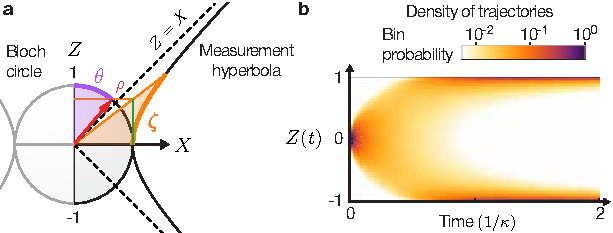
\includegraphics[scale=1.4]{mthry/CircleHyperbola}
\par\end{centering}
\caption[Random walk on the measurement hyperbola.]{\textbf{Random walk on the measurement hyperbola.\label{fig:Random-walk-on-hyperb}
a,} Circular and hyperbolic geometric representations of the pure
qubit state, $\rho$, parametrized by the circular and hyperbolic
angles $\theta$ and $\zeta$, respectively, obeying $\cos\left(\theta\right)=\tanh\zeta$.
The circle depicts a slice though the XZ plane of the Bloch sphere,
which is well-suited to represent unitary dynamics. The random walk
of $\zeta$ due to the measurement takes place on the unit hyperbola,
with asymptotes defined by the lines $Z=\pm X$. \textbf{b,} Histogram
of quantum trajectory densities obtained from simulations of the flying-spin
model. All trajectories (not shown here) begin with the initial state
defined by the Bloch coordinates $X\left(0\right)=1$ and $Z\left(0\right)=0$.
The time axis is scaled in units of the measurement rate, $\kappa$.
}
\end{figure}

The circular and hyperbolic coordinate transformations together with
Eqs.~(\ref{eq:SpinBathHRabi}) and~(\ref{eq:HyperbolicRotationMsr})
can be employed to construct a finite-difference numerical scheme
to calculate the quantum trajectory of the qubit subject to homodyne
monitoring. Notably, since the difference equations were derived \emph{without}
approximations, especially with regard to the size of $\Delta t$,
they guarantee a physical system state for all parameters and at all
time, features which offer some practical advantages for numerical
simulations. In the following subsection, Sec.~\ref{subsec:Continuous-limit:-Wiener},
we construct the continuum limit of the model and formally derive
the differential equations for the quantum trajectory of the qubit.


\subsection{Continuum limit: Wiener noise and stochastic calculus\label{subsec:Continuous-limit:-Wiener}}

In this section, we take the appropriate limit in which the measurement
becomes continuous. In this limit, the interaction time, $\Delta t$,
becomes infinitely small while the measurement strength, $\lambda$,
becomes infinitely large. Since each short sequence of individual
measurements carries an infinitesimal amount of information in this
limit, we coarse-grain the measurement record in the following way.
The evolution up to time $t$ is divided in $m$ intervals of total
duration $\dt$, while each of these intervals is further subdivided
in $l$ yet smaller intervals, each of duration $\Delta t$; i.e.,
$t=n\Delta t=ml\Delta t$ and $\dt=l\Delta t$. The interaction amplitude,
$\lambda$, is chosen to be $\lambda=\sqrt{\kappa/\Delta t}$, where
$\kappa$ denotes the interaction rate. Subject to appropriate scaling,
by a factor $\sqrt{\Delta t}$, the sum of all measurement results
up to time $t$ is the measurement signal $J_{t}=\sqrt{\Delta t}\sum_{m'=0}^{m}\sum_{l'=0}^{l}r_{m'l'}$.
During a time interval $\dt$, beginning at $t=ml\Delta t$ and ending
at $t'=\left(m+1\right)l\Delta t$, the signal changes by 
\begin{equation}
\mathrm{d}J_{t}=J_{\left(m+1\right)l\Delta t}-J_{ml\Delta t}=\sqrt{\Delta t}\sum_{k=ml}^{\left(m+1\right)l}r_{k}\:.\label{eq:dJ-stoch-diff-eq}
\end{equation}
Equation~(\ref{eq:dJ-stoch-diff-eq}) is known as a \emph{stochastic
difference equation, }because the difference increment in the variable
$J_{t}$ is a random variable. Assuming the state of the system does
not appreciably change over the time interval $\dt$, the measurement
results, $r_{k}$, are independent and identically distributed binary
random variables described by the probability function $\wp\left[r_{k}\right]=\frac{1}{2}\left(1-\epsilon r_{k}Z\left(t\right)\right),$
recall Eq.~(\ref{eq:PflyingSpinPM1}), where $\epsilon=\sqrt{\kappa\Delta t}$.
It follows that the mean and variance of the measurement increment
are 
\begin{align}
\E{\mathrm{d}J_{t}} & =l\sqrt{\Delta t}\E{r_{k}}=-\sqrt{\kappa}Z\left(t\right)\dt\,,\label{eq:EdJ-qubithomo}\\
\mathrm{Var}\left[\mathrm{d}J_{t}\right]= & l\Delta t\mathrm{Var}\left[r_{k}\right]\approx\dt\,,\label{eq:Var-dJ-qubithomo}
\end{align}
respectively, while, according to the central limit theorem, all higher-order
cumulants of the probability distribution for $\mathrm{d}J_{t}$ vanish
in the limit of large $l$. Working in this limit, and employing Eqs.~(\ref{eq:EdJ-qubithomo})
and~(\ref{eq:Var-dJ-qubithomo}), the stochastic difference equation,
Eq.~(\ref{eq:dJ-stoch-diff-eq}), can be taken to  the continuum
limit,\footnote{For completeness, we note that Eq.~(\ref{eq:QubitHomo:dJ}) is a
special case of Eq.~(\ref{eq:Jhom}). }

\begin{equation}
\boxed{\mathrm{d}J\left(t\right)=-\sqrt{\kappa}Z\left(t\right)\dt+\dW\left(t\right)\,},\label{eq:QubitHomo:dJ}
\end{equation}
where the infinitesimal term $\dW\left(t\right)$ represents Gaussian
white noise, and is known as the \emph{Wiener increment}. It obeys
the following canonical relations and probability density: 
\begin{align}
\E{\dW\left(t\right)} & =0\,, & \dW\left(t\right)\dt & =0\,,\label{eq:dW-relation-1}\\
\E{\dW\left(t\right)^{2}} & =\dt\,, & \wp\left(\dW\right) & =\frac{\exp\left(-\dW^{2}/(2\dt)\right)}{\sqrt{2\pi\dt}}\,.\label{eq:dW-relation-2}
\end{align}


\paragraph{Stochastic calculus. }

Equation~(\ref{eq:QubitHomo:dJ}) is known as a\emph{ stochastic
differential equation} (SDE) because the infinitesimal differential
is not completely determined, but is a random variable. Notably, in
obtaining this equation, we took the value of the function $Z\left(t\right)$
at the \emph{beginning} of the timestep $\dt$. In general, because
the stochastic noise is not smooth and not differentiable if we had
taken the value of the function at the\emph{ end} of the time-interval
$\dt$ we would have obtained a different form of the SDE. By taking
the value of the function at the beginning of the timestep, the SDE
we obtained is said to be in \emph{Itô form}; otherwise, it would
have been in \emph{Stratonovich form}. The two forms are not equivalent
in a straightforward manner, but for our purposes, it will suffice
to only consider the Itô form; see Chapter~3 of Ref.~\citet{Jacobs2010Book}
for an in-depth discussion. From Eqs.~(\ref{eq:dW-relation-1}) and
(\ref{eq:dW-relation-2}) it follows that the SDE solution only depends
on terms proportional to $\dt,$ $\dW,$ and $\dW^{2},$ while all
other terms of the form $\dt^{p}\dW^{q}$ are vanishing. Importantly,
in an unusual departure from the rules of differential calculus, in
the continuum limit, one can set $\dW^{2}=\dt$, a result known as
\emph{Itô}'s \emph{rule}. We note that $\dW\left(t\right)$ is an
idealized Gaussian noise process in that it has a perfect delta function
correlation in time, which implies its Markovianity, but also that
it has a white noise power spectral density, non-zero for \emph{all}
frequencies.


\paragraph{Itô SDE for the Bloch vector. }

In our example, the Bloch vector of the qubit can be parameterized\footnote{For simplicity, we have assumed $X\left(t\right)>0$ for all $t$.}
by its Z component, $\vec{S}\left(t\right)=\left(\sqrt{1-Z\left(t\right)^{2}},0,Z\left(t\right)\right)^{\intercal}$.
Thus, it suffices to derive an SDE for $Z\left(t\right)$, which is
obtained from the system state, $\ket{\psi_{J}\left(t\right)}$, conditioned
on the measurement signal $J\left(t\right)$ by taking the expectation
value of $\hat{\sigma}_{z}$, $Z\left(t\right)=\braOket{\psi_{J}\left(t\right)}{\hat{\sigma}_{z}}{\psi_{J}\left(t\right)}$.
The SDE is derived by first Taylor expanding $Z\left(t\right)=\cos\left(\theta\left(t\right)\right)$
to first order in $\dt$, $\mathrm{d}Z\left(t\right)\approx-\sqrt{1-Z\left(t\right)^{2}}\mathrm{d}\theta\left(t\right)-\frac{1}{2}Z\left(t\right)\mathrm{d}\theta\left(t\right)^{2}$,
where we have retained terms to second order in $\mathrm{d}\theta\left(t\right)$.
This is necessary because $\mathrm{d}\theta\left(t\right)$, recalling
Eq.~(\ref{eq:SPinBath:ThPM}), is proportional to $\dW$, and $\dW^{2}=\dt$.
By summing $l$ times over the difference equation and performing
the same coarse graining employed to arrive at Eq.~(\ref{eq:QubitHomo:dJ}),
we arrive at the Itô form of the SDE for the Z component of the Bloch
vector of a qubit subject to heterodyne monitoring of $\hat{\sigma}_{z}$,
\begin{equation}
\boxed{\mathrm{d}Z\left(t\right)=-\sqrt{\kappa}\left(1-Z\left(t\right)^{2}\right)\dW\left(t\right)\,.}\label{eq:QubitHomoToyConti}
\end{equation}
Equation~(\ref{eq:QubitHomoToyConti}) is a non-linear diffusion
equation with a state-dependent diffusion coefficient, $D\left(Z\right)=\kappa\left(1-Z^{2}\right)^{2}$,
which is maximized for $Z\left(t\right)=0$, but approaches zero for
$Z=\pm1$. Mathematically, it is for this reason, that in the limit
$t\rightarrow\infty$, the system tends to one of the pointer states
($Z=\pm1$) of the measurement, where diffusion vanishes, and states
cluster. 


\section{Quantum trajectory theory \label{sec:Quantum-trajectory-theory}}

The preceding sections introduced the general background required
to develop quantum trajectory theory. With the aid of specific examples,
important overriding themes were highlighted, which will carry us
forward in this section, and play a key role in understanding photon-counting,
homodyne, and heterodyne measurements. 


\subsection{Photodetection \label{subsec:Photodetection}}

Photodetection is the minimal time-continuous measurement scheme —
at each moment in time, the detector records one of only two possible
results: $r=0$ (``no-click'') or $r=1$ (``click''). As discussed
in Sec.~\ref{sec:Introductory-example:-qubit}, the measurement result
communicates some knowledge about the system state and the unavoidable
disturbance caused to it by the measurement itself.\footnote{From an operational point of view, the state of the system is strictly
speaking only \emph{our} knowledge about the probabilities for outcomes
of \emph{future} measurements of the system.} The information gain as well as the action of the disturbance are
encoded in the measurement operators, $\hat{M}_{r}$, recall Eq.~(\ref{eq:MrSpinBath}).
These operators, also known as Kraus operators, generalize unitary
evolution due to a system Hamiltonian, $\hat{H}$, so as to include
the effect of the measurement process. Microscopically, the measurement
operators, $\hat{M}_{r}$, can be understood to describe the unitary
interaction between the system and another, auxiliary one, which is
subsequently measured by a von Neumann measurement apparatus, see
discussion on Neumark's theorem in Sec.~\ref{sec:Introductory-example:-qubit}.
In this section, we will only concern ourselves with the system evolution
subject to measurement, and will make no further reference to the
auxiliary system, other than to specify the system operator $\hat{c}$
that couples the two. The minimal set of infinitesimal measurement
operators, which corresponding to the no-click ($r=0$) and click
($r=1$) evolution, are
\begin{align}
\hat{M}_{0}\left(\dt\right) & =\hat{1}-\left(\half\hat{c}^{\dagger}\hat{c}+i\hat{H}\right)\dt\,,\label{eq:photonM0}\\
\hat{M}_{1}\left(\dt\right) & =\sqrt{dt}\hat{c}\,,\label{eq:photonM1}
\end{align}
in units where $\hbar=1$. One can verify that $\hat{M}_{0}\left(\dt\right)$
and $\hat{M}_{1}\left(\dt\right)$ form a positive-operator-valued
measure (POVM) on the space of results. Hence, they form a resolution
of the identity, $\hat{M}_{0}^{\dagger}\left(\dt\right)\hat{M}_{0}\left(\dt\right)+\hat{M}_{1}^{\dagger}\left(\dt\right)\hat{M}_{1}\left(\dt\right)=\hat{1}+\mathcal{O}\left(\dt^{2}\right)$,
guaranteeing that the law of total probability is satisfied, i.e.,
a measurement yields an outcome with probability 1. The probability
for a specific outcome, $r=0$ or $r=1$, is is given by the generalized
measurement postulate, Eq.~(\ref{eq:GenMsrPosProb}), $\wp_{r}\left(\dt\right)=\left\langle \hat{M}_{r}^{\dagger}\left(\dt\right)\hat{M}_{r}\left(\dt\right)\right\rangle $,
\begin{align}
\wp_{0}\left(\dt\right) & =1-\dt\left\langle \hat{c}^{\dagger}\hat{c}\right\rangle +\mathcal{O}\left(\dt^{2}\right)\,,\label{eq:PhotonP0}\\
\wp_{1}\left(\dt\right) & =\dt\left\langle \hat{c}^{\dagger}\hat{c}\right\rangle \,.\label{eq:PhotonP1}
\end{align}
We define the time-continuous photodetection measurement record to
be the number of photodetections up to time $t$, denoted $N\left(t\right)$.
It follows that the infinitesimal measurement increment, denoted $\dN\left(t\right)$,
is a \emph{point-process}, also known as the \emph{Poisson process},
defined by 
\begin{align}
\dN\left(t\right)^{2} & =\dN\left(t\right)\,,\label{eq:Photon-dN-2}\\
\E{\dN\left(t\right)} & =\wp_{1}\left(\dt\right)\,,\label{eq:Photon-dN-E}
\end{align}
where $\E{\cdot}$ denotes the expectation value in the classical
sense, see Sec.~\ref{subsec:Classical-measurement-theory-basic-concept}.
In the continuum limit, the detector photocurrent, $I\left(t\right)=\dN\left(t\right)/\dt$,
consists of a series of Dirac $\delta$-functions at the times of
the clicks. 

\paragraph{Stochastic master equation (SME) for ideal photodetection. }

Ideal photodetection is the limit where the photodetector collects
the entirety of the system output field and adds no technical noise,
i.e., the quantum measurement efficiency is one, $\eta=1$. According
to the generalized projection postulate, Eq.~(\ref{eq:GenMsrPosProj}),
the state of the system after a measurement at time $t$ conditioned
on the measurement result $r=0$ or $r=1$ is 
\begin{equation}
\rho_{r}\left(t+\dt\right)=\frac{\hat{M}_{r}\left(\dt\right)\rho\left(t\right)\hat{M}_{r}^{\dagger}\left(\dt\right)}{\wp_{r}\left(\dt\right)}\,.\label{eq:click:rhoPLUS}
\end{equation}
In the continuum limit, where the instantaneous measurement outcome
is the photocurrent $I\left(t\right),$ the two possible states, $\rho_{0}\left(t+\dt\right)$
and $\rho_{1}\left(t+\dt\right)$, can be combined in a single stochastic
differential equation (SDE) for the posterior system state $\rho_{I}\left(t+\dt\right)$
conditioned on $I\left(t\right)$, resulting in the state differential,
in Itô form,
\begin{align}
\mathrm{d}\rho_{I}\left(t\right) & =\rho_{I}\left(t+\dt\right)-\rho_{I}\left(t\right)\\
 & =\dN\left(t\right)\left(\rho_{1}\left(t+\dt\right)-\hat{1}\right)+\left(1-\dN\left(t\right)\right)\left(\rho_{0}\left(t+\dt\right)-\hat{1}\right)\,,\label{eq:SME-prior}
\end{align}
which can be simplified by Taylor expanding the denominator of $\rho_{0}\left(t+\dt\right)$,
retaining terms to order $\dt$, and employing the stochastic calculus
rule\footnote{Technically, $\dN\left(t\right)\dt$ is not strictly zero. However,
because the mean of $\dN$ is infinitesimal, $\dN\left(t\right)$
is negligible when compared with $\dt$, and so are all higher-order
products containing both $\dN$ and $\dt$. }
\begin{equation}
\dN\left(t\right)\dt=0\,
\end{equation}
in order to obtain the \emph{stochastic master equation} (SME) for
photodetection, in the Schrödinger picture and in Itô form,
\begin{equation}
\boxed{\mathrm{d}\rho_{I}\left(t\right)=\left(\dN\left(t\right)\mathcal{G}\left[\hat{c}\right]+\dt\mathcal{H}\left[\hat{H}_{\mathrm{eff}}\right]\right)\rho_{I}\left(t\right)\,,}\label{eq:photon:SME}
\end{equation}
where the superoperators $\mathcal{G}\left[\hat{c}\right]\rho$ and
$\mathcal{H}\left[\hat{c}\right]\rho$ are defined by
\begin{align}
\mathcal{G}\left[\hat{c}\right]\rho\equiv & \frac{\hat{c}^{\dagger}\rho\hat{c}}{\Tr{\hat{c}^{\dagger}\rho\hat{c}}}-\rho\,,\label{eq:PhotoG}\\
\mathcal{H}\left[\hat{c}\right]\rho\equiv & \hat{c}\rho+\rho\hat{c}^{\dagger}-\Tr{\hat{c}\rho+\rho\hat{c}^{\dagger}}\rho\label{eq:PhotoH}\\
= & \left(\hat{c}-\left\langle \hat{c}\right\rangle \right)\rho+\rho\left(\hat{c}^{\dagger}-\left\langle \hat{c}^{\dagger}\right\rangle \right)\,,
\end{align}
The superoperator $\mathcal{G}$ results in point-like discontinuous
state evolution, while $\mathcal{H}$ results in smooth, continuous,
but non-unitary evolution generated by the effective non-Hermitian
Hamiltonian 
\begin{equation}
\hat{H}_{\text{eff}}\equiv\hat{H}-i\frac{1}{2}\hat{c}^{\dagger}\hat{c}\,.\label{eq:H_eff_noclick}
\end{equation}
Notably, the trace terms in Eqs.~(\ref{eq:PhotoG}) and (\ref{eq:PhotoH})
make the photodetection SME, Eq.~(\ref{eq:photon:SME}), \emph{nonlinear}
in the state density, $\rho_{I}$. The origin of the trace term in
$\mathcal{H}$, namely $\Tr{\hat{c}\rho+\rho\hat{c}^{\dagger}}$,
is the Taylor expansion of the denominator of Eq.~(\ref{eq:click:rhoPLUS}),
which gives the no-click probability, $\wp_{0}\left(\dt\right)$.
As discussed in Sec.~\ref{sec:Introductory-example:-qubit}, the
role of this term is to preserve the state density trace for all time,
$\Tr{\rho_{I}\left(t\right)}=1$. The solution of the SME is a stochastic
path taken by the conditional state over time, known as a \emph{quantum
trajectory}, a term\emph{ }coined in Ref.\emph{~\citet{Carmichael1993}. }

\paragraph{Stochastic Schrödinger equation (SSE) for photodetection. }

For a system in a pure state, $\rho_{I}\left(t\right)=\kb{\psi_{I}\left(t\right)}{\psi_{I}\left(t\right)}$,
the SME, Eq.~(\ref{eq:photon:SME}), preserves the purity of the
state for all times. It follows that the state evolution is described
by a type of Schrödinger equation, known as the \emph{stochastic Schrödinger
equation }(SSE), 
\begin{equation}
\boxed{\mathrm{d}\ket{\psi_{I}\left(t\right)}=\left[\dt\left(\frac{\left\langle \hat{c}^{\dagger}\hat{c}\right\rangle \left(t\right)}{2}-\frac{\hat{c}^{\dagger}\hat{c}}{2}-i\hat{H}\right)+\dN\left(t\right)\left(\frac{\hat{c}}{\sqrt{\left\langle \hat{c}^{\dagger}\hat{c}\right\rangle \left(t\right)}}-\hat{1}\right)\right]\ket{\psi_{I}\left(t\right)}\,,}\label{eq:SSE-click}
\end{equation}
which is nonlinear in the state $\ket{\psi_{I}\left(t\right)}$. The
non-linear terms contain the expectation value $\left\langle \hat{c}^{\dagger}\hat{c}\right\rangle \left(t\right)=\frac{1}{2}\braOket{\psi_{I}\left(t\right)}{\hat{c}^{\dagger}\hat{c}}{\psi_{I}\left(t\right)}$,
which gives the click probability $\wp_{1}$, see Eq.~(\ref{eq:PhotonP1}).
Because these non-linear terms render analytic treatment of the equations
particularly difficult in general, a linear description of the state
evolution is desired, and can be accomplished as described next. The
term $\frac{1}{2}\dt\left\langle \hat{c}^{\dagger}\hat{c}\right\rangle \left(t\right)\ket{\psi_{I}\left(t\right)}$,
which updates the observer's state-of-knowledge in a non-linear way,
mathematically, ensures the proper normalization of $\ket{\psi_{I}\left(t\right)}$
for all times; however, normalization need not be enforced for each
infinitesimal timestep $\dt$. Instead, it can ``manually'' be enforced
for the no-click periods, $I\left(t\right)=0$, by first first solving
for the un-normalized system state, denoted with a tilde, $\ket{\tilde{\psi}_{I=0}\left(t\right)}$,
then normalizing it, $\ket{\psi_{I=0}\left(t\right)}=\ket{\tilde{\psi}_{I=0}\left(t\right)}/\braket{\tilde{\psi}_{I=0}\left(t\right)}{\tilde{\psi}_{I=0}\left(t\right)}$,
where the effective Schrödinger equation for $\ket{\tilde{\psi}_{I=0}\left(t\right)}$
is
\begin{equation}
\boxed{i\frac{\mathrm{d}}{\dt}\ket{\tilde{\psi}_{I=0}\left(t\right)}=\hat{H}_{\mathrm{eff}}\ket{\tilde{\psi}_{I=0}\left(t\right)}\,,}\label{eq:SSE-click-1}
\end{equation}
where $\hat{H}_{\mathrm{eff}}$ is the non-Hermitian Hamiltonian,
Eq.~(\ref{eq:H_eff_noclick}). Since Eq.~(\ref{eq:SSE-click-1})
is linear, it is generally easier to solve for the time-dynamics.
Calculation of system averages still requires normalizing $\ket{\tilde{\psi}_{I=0}\left(t\right)}$
by its the state norm, $\braket{\tilde{\psi}_{I}\left(t\right)}{\tilde{\psi}_{I}\left(t\right)}$,
which gives the probability of no-clicks occurring for duration $t$.
We remark that Eq.~(\ref{eq:SSE-click-1}) corresponds to tracking
the sub-ensemble of quantum trajectories that contain no clicks, or
mathematically, to the repetitive application of the measurement operator
$\hat{M}_{0}$; hence, in general, in the limit $t\rightarrow\infty$,
it leads to the decay of the norm to zero. 

\paragraph{Unconditioned evolution: master equation for photodetection. }

By averaging over all possible evolutions due to all measurement outcomes
at each instant, one can obtain the \emph{unconditioned} evolution
of the quantum state, denoted $\rho\left(t+\dt\right)$, from Eq.~(\ref{eq:photon:SME}).
Simplifying the average, $\rho\left(t+\dt\right)=\sum_{r}\wp_{r}\rho_{r}\left(t+\dt\right)$,
\begin{align}
\rho\left(t+\dt\right) & =\hat{M}_{0}\left(\dt\right)\rho\hat{M}_{0}^{\dagger}\left(\dt\right)+\hat{M}_{1}\left(\dt\right)\rho\hat{M}_{1}^{\dagger}\left(\dt\right)\\
 & =\rho\left(t\right)-i\left[\hat{H},\rho\left(t\right)\right]\dt+\mathcal{D}\left[\hat{c}\right]\rho\left(t\right)\dt\,,\label{eq:MEforPhootdetection}
\end{align}
where the superoperator $\mathcal{D}$ is defined to be 
\begin{equation}
\mathcal{D}\left[\hat{c}\right]\rho\equiv\hat{c}\rho\hat{c}^{\dagger}-\frac{1}{2}\left\{ \hat{c},\rho\right\} _{+}\,.\label{eq:LindbladSuperop}
\end{equation}
Eq.~(\ref{eq:MEforPhootdetection}) for the unconditioned state evolution
is known as the \emph{master equation, }in Lindblad\emph{ }form \citep{lindblad1976}.\footnote{For a comprehensive summary of the properties of the master equation
and Lindbladians, see Refs.~\citet{AlbertVV2014-Lindblad,Albert2016-Lindblad}.} Unlike the SME, it is linear in the state density, $\rho$, and yields
deterministic state evolution, since there are no stochastic increments,
$\dN$ or $\dW$. Notably, the master equation is very general and
makes no reference to photodetection, other than specifying the system
operator $\hat{c}$ subject to detection, although it does not specify
how. As will be evident from the following section, the same master
equation is obtained for heterodyne detection of $\hat{c}$, see Sec.~\ref{subsec:Homodyne-and-heterodyne}.
The two SMEs corresponding to the same master equation are known as
\emph{unravellings}\footnote{The\emph{ }term 'unraveling' was coined in Ref. \citet{Carmichael1993}.}\emph{
}of it. We note that the unravellings of the master equation are not
unique.

\subparagraph{Imperfect detection.}

Imperfect conditions limit the observer's access to information regarding
the system and generally result in excess noise. The effect of imperfections
can be modeled by considering an ideal photodetector that is, however,
sensitive to only a fraction $\eta$ of the system output field. This
fraction, known as the \emph{quantum measurement efficiency}, is a
real number between zero and one, $0\leq\eta\leq1$. Because of the
loss of information due to imperfect detection, over time, the system
state will, in general, become mixed, with purity less than one, $0\leq\Tr{\rho^{2}}<1$.
To account for the imperfections, SME, Eq.~(\ref{eq:photon:SME}),
is be modified in the following way, see Sec.~4.8.1 of Ref.~\citet{wiseman2010book}:

\begin{equation}
\boxed{\mathrm{d}\rho_{I}\left(t\right)=\left(\dN\left(t\right)\mathcal{G}\left[\sqrt{\eta}\hat{c}\right]+\dt\mathcal{H}\left[-i\hat{H}-\eta\frac{1}{2}\hat{c}^{\dagger}\hat{c}\right]+\dt\left(1-\eta\right)\mathcal{D}\left[\hat{c}\right]\right)\rho_{I}\left(t\right)\,,}\label{eq:photon:SME-loss}
\end{equation}
where the jump probability for each timestep is obtained by also replacing
$\hat{c}$ with $\sqrt{\eta}\hat{c}$ in Eq.~(\ref{eq:Photon-dN-E}),
$\E{\dN\left(t\right)}=\eta\Tr{\hat{c}^{\dagger}\hat{c}\rho}\dt$.
Considering the two limits $\eta\rightarrow0$ and $\eta\rightarrow1$,
one can associate the Lindblad superoperator $\mathcal{D}$ with information
loss, and $\mathcal{H}$ and $\mathcal{G}$ with information gain
due to the measurement.


\subsection{Homodyne and heterodyne detection\label{subsec:Homodyne-and-heterodyne}}

The measurements described so far are not sensitive to the phase of
the system output field, but only its amplitude. In the following,
we describe \emph{dyne} measurements\emph{, homodyne} or \emph{heterodyne,
}which provide information about the phase and a qualitatively different
(diffusive) trajectory unraveling.

\paragraph{Physical implementation. }

Dyne detection is realized by mixing the system output signal with
a local-oscillator (LO) tone, see Fig.~\ref{fig:Schematic-representation-of}.
For a system carrier frequency, conventionally termed the radio frequency
(RF), $\omega_{\mathrm{RF}}$ and LO frequency $\omega_{\mathrm{LO}}$,
the lower sideband of the mixed-signal is at intermediate frequency
(IF), $\omega_{\mathrm{IF}}=\omega_{\mathrm{LO}}-\omega_{\mathrm{RF}}$.
In homodyne detection, the LO is tuned in resonance with the system
carrier, resulting in a direct-current (DC) IF signal, $\omega_{\mathrm{IF}}=0$,
proportional to a quadrate of the RF signal that depends on the LO
phase. The IF signal is typically sampled and digitally processed.
On the other hand, in heterodyne detection, the LO frequency is significantly
detuned from the RF, $\omega_{\mathrm{IF}}\gg0$, resulting in a an
oscillatory IF signal, which is demodulated to extract the information-bearing
\emph{in-quadrature} (I) and \emph{out-of-quadrature }(Q) components.
Note that the heterodyne measurement record consists of a series of
not one but \emph{ two} values, I and Q. Heterodyne detection is equivalent
to two concurrent homodyne detections with LO phases $90^{\circ}$
apart. 

\begin{figure}
\begin{centering}
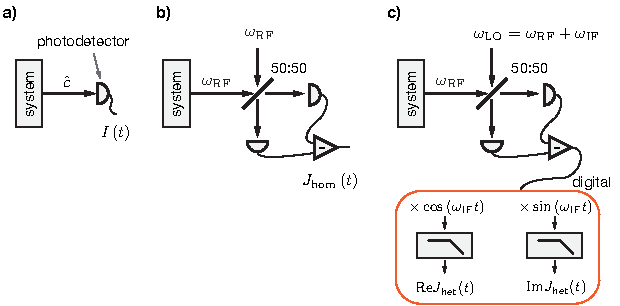
\includegraphics[scale=1.4]{mthry/Heterodyne2}
\par\end{centering}
\caption[Schematic representations of a photo, homodyne, and heterodyne detection
schemes.]{\label{fig:Schematic-representation-of}Schematic representations
of a (a) photo, (b) homodyne, and (c) heterodyne detection schemes.
\textbf{a, }The system output field, proportional to the system coupling
operator $\hat{c}$, is directly monitored with a photodetector, whose
photocurrent $I\left(t\right)$ is the measurement record. \textbf{b,}
Optical balanced homodyne detection: system output field, assumed
with carrier frequency $\omega_{\mathrm{RF}}$, is interfered on a
50:50 beam splitter with a strong local oscillator (LO) tone at the
carrier frequency, $\omega_{\mathrm{LO}}=\omega_{\mathrm{RF}}$. The
measurement record, $J_{\mathrm{hom}}\left(t\right)$, is obtained
from the  difference of the photodetector currents on each output
arm of the beamsplitter. \textbf{c,} Balanced heterodyne detection
scheme (with digital demodulation): LO frequency is detuned by an
intermediate frequency value, $\omega_{\mathrm{IF}},$ where $\omega_{\mathrm{IF}}\ll\omega_{\mathrm{RF}},\omega_{\mathrm{LO}}$.
The difference of the photodetector currents of each arm, which oscillates
at $\omega_{\mathrm{IF}}$, is digitally demodulated to obtain the
in-phase {[}out-of-phase{]} quadrature $\mathrm{Re}J_{\mathrm{het}}\left(t\right)$
{[}$\mathrm{Im}J_{\mathrm{het}}\left(t\right)${]} by digitally mixing
the signal with a reference one, $\cos\left(\omega_{\mathrm{IF}}t\right)$
{[}$\sin\left(\omega_{\mathrm{IF}}t\right)${]}, and low-pass filtering
the output to reject tones above $\omega_{\mathrm{IF}}$. Digital
panel schematic inspired by Ref.~\citep{Campagne2016-Fluorescence}.
}
\end{figure}


\paragraph{Homodyne measurement record. }

The homodyne measurement signal is mathematically described by a function,
$J_{\mathrm{hom}}\left(t\right)$, that is real and continuous everywhere
but differentiable nowhere, see Sec.~\ref{subsec:Continuous-limit:-Wiener}.
The measurement signal gradually reveals information about a system
operator of the form $\hat{c}+\hat{c}^{\dagger}$, where $\hat{c}$
is the operator coupled to the measurement apparatus, which for the
example of Sec.~\ref{subsec:Continuous-limit:-Wiener} is $\hat{c}=-\frac{\sqrt{\kappa}}{2}\hat{\sigma}_{z}$.
In Itô form, the measurement increment is
\begin{equation}
\mathrm{d}J_{\mathrm{hom}}\left(t\right)=\left\langle \hat{c}+\hat{c}^{\dagger}\right\rangle \left(t\right)\dt+\dW\left(t\right)\,,\label{eq:Jhom}
\end{equation}
where $\dW\left(t\right)$ is the stochastic Wiener increment satisfying
the canonical relations given in Eqs.~(\ref{eq:dW-relation-1})
and~(\ref{eq:dW-relation-2}).

\paragraph{Heterodyne measurement record. }

The heterodyne measurement signal consists of two functions: the in-phase,
$J_{I}\left(t\right)$, and out-of-phase, $J_{Q}\left(t\right)$,
quadrature functions, which can be combined in a single complex function,
$J_{\mathrm{het}}\left(t\right)\equiv\frac{1}{2}\left(J_{I}\left(t\right)+iJ_{Q}\left(t\right)\right)$,
continuous everywhere but differentiable nowhere.  In heterodyne
detection, $J_{\mathrm{het}}\left(t\right)$ gradually reveals information
about a system operator $\hat{c}$, which need not be Hermitian but
which can be decomposed into the sum of two Hermitian operators, corresponding
to two observables, know as the quadrature operators, 
\begin{equation}
\hat{I}\equiv\hat{c}+\hat{c}^{\dagger}\ \text{and}\ \hat{Q}\equiv-i\left(\hat{c}-\hat{c}^{\dagger}\right)\,,
\end{equation}
so that $\hat{c}=\frac{1}{2}\left(\hat{I}+i\hat{Q}\right)$. The Itô
form of the measurement increment is 
\begin{equation}
\mathrm{d}J_{\mathrm{het}}\left(t\right)=\left\langle \hat{c}\right\rangle \left(t\right)\dt+\dZ\left(t\right)\,,\label{eq:Jhet-perfect}
\end{equation}
where $\dZ\equiv\frac{1}{\sqrt{2}}\left(\dW_{I}\left(t\right)+i\dW_{Q}\left(t\right)\right)$
is the complex Wiener increment, the sum of two independent Wiener
increments, $\dW_{I}\left(t\right)$ and $\dW_{Q}\left(t\right)$,
that satisfy $\E{\dW_{I}\left(t\right)\dW_{Q}\left(t\right)}=0$,
so that $\dZ\left(t\right)^{*}\dZ\left(t\right)=\dt$ and $\dZ\left(t\right)^{2}=0$.
We note that $\dZ$ is obtained by making the substitution $e^{i\omega_{{\rm RF}}t}\dW\rightarrow\dZ$
in the heterodyne derivation.

For concreteness, consider the example of a qubit coupled to the environment
where an observer performs heterodyne detection of the qubit fluoresce
\citep{Campagne-Ibarcq2014,Campagne2016-Fluorescence,Naghiloo2016}.
The system-environment coupling is given by the non-Hermitian operator
$\hat{c}=\hat{\sigma}_{-}\equiv\kb{+z}{-z}$, which is decomposed
into the two Hermitian quadrature operators $\hat{I}=\hat{\sigma}_{x}$
and $\hat{Q}=-\hat{\sigma}_{y}$. Note the minus sign in $\hat{Q}$.
The heterodyne detection of $\hat{\sigma}_{-}$ can be understood
as a homodyne detection of the observable $\hat{I}$ and a concurrent
homodyne detection of the observable $\hat{Q}$, each with efficiency
$\eta=1/2$, see below. Consider the example where the qubit is replaced
by a cavity, the coupling operator is $\hat{c}=\hat{a}$, where $\hat{a}$
is the annihilation operator, and the whose cavity output field is
subject to heterodyne monitoring, which reveals information about
$\hat{I}=\hat{a}+\hat{a}^{\dagger}$ and $\hat{Q}=-i\left(\hat{a}-\hat{a}^{\dagger}\right)$.
For a coherent state in the cavity, $\ket{\alpha\left(t\right)}$,
the measurement record gradually reveals its complex amplitude, $\E{\mathrm{d}J_{\mathrm{het}}\left(t\right)/\dt}=\braOket{\alpha\left(t\right)}{\frac{1}{2}\left(\hat{I}+\hat{i}\hat{Q}\right)}{\alpha\left(t\right)}=\alpha\left(t\right)$. 

\paragraph{Measurement operators and the SME for perfect dyne detection.}

At an instant in time, the noisy heterodyne record, $J_{\mathrm{het}}\left(t\right)$,
relates the measurement outcome to the quantum trajectory evolution
according to the action of the measurement operator (see discussion
on Pg.~\pageref{eq:MrSpinBath})
\begin{equation}
\hat{M}_{J}=\hat{1}-i\hat{H}\dt-\frac{1}{2}\hat{c}^{\dagger}\hat{c}\dt+J_{\mathrm{het}}^{*}\left(t\right)\hat{c}\dt\,.\label{eq:hetero:msrmap}
\end{equation}
The measurement operator for homodyne detection, also denoted $\hat{M}_{J}$,
is obtained by making the substitution $J_{\mathrm{het}}^{*}\left(t\right)\rightarrow J_{\mathrm{hom}}\left(t\right)$
in Eq.~(\ref{eq:hetero:msrmap}). Notably, the non-orthogonal set
of measurement operators for dyne detection, $\left\{ \hat{M}_{J}:J\right\} $,
is continuous, in contrast with that of photodetection, which consists
of two elements, $\left\{ \hat{M}_{0},\hat{M}_{1}\right\} ,$ since
there are only two possible measurement outcomes, click or no click.
The system state conditioned on the record at time $t$, denoted $\rho_{J}$,
is obtained by employing the generalized measurement postulate, Eq.~(\ref{eq:GenMsrPosProj}),

\begin{equation}
\rho_{J}\left(t+\dt\right)=\frac{\hat{M}_{J}\rho_{J}\left(t\right)\hat{M}_{J}^{\dagger}}{\Tr{\hat{M}_{J}\rho_{J}\left(t\right)\hat{M}_{J}^{\dagger}}}\,.\label{eq:click:rhoPLUS-1}
\end{equation}
Equation~(\ref{eq:click:rhoPLUS-1}) is simplified by Taylor expanding
the denominator to order $\dt$ and writing the infinitesimal state
change, in Itô form, $\mathrm{d}\rho_{J}\left(t\right)=\rho_{J}\left(t+\dt\right)-\rho_{J}\left(t\right)$,
thus obtaining the SME for perfect heterodyne detection, in the Schrödinger
picture,
\begin{equation}
\mathrm{d}\rho_{J}\left(t\right)=\left[-i\dt[\hat{H},\cdot]+\dt\mathcal{D}[\hat{c}]+\dZ^{*}\left(t\right)\mathcal{H}[\hat{c}]\right]\rho_{J}\left(t\right)\,,\label{eq:SME-Heterodyne}
\end{equation}
where the superoperators $\mathcal{D}$ and $\mathcal{H}$ are defined
in Eqs.~(\ref{eq:LindbladSuperop}) and~(\ref{eq:PhotoH}), respectively.
Equation~(\ref{eq:SME-Heterodyne}) has to be solved jointly with
Eq.~(\ref{eq:Jhet-perfect}). The homodyne SME is obtained by making
the substitution $\dZ^{*}\left(t\right)\rightarrow\dW\left(t\right)$
in Eq.~(\ref{eq:SME-Heterodyne}).  

\paragraph{SME for imperfect measurements.}

Measurement imperfections (see discussion on Pg.~\ref{eq:photon:SME-loss})
are primarily due to: i) losses associated with the propagation of
the system output field to the measurement apparatus, characterized
by a quantum efficiency $\eta_{\mathrm{prop}}$, and ii) finite detector
efficiency, $\eta_{\mathrm{det}}$. The measurement chain efficiency
is given by the product of those of it sub-components, $\eta=\eta_{\mathrm{prop}}\eta_{\mathrm{det}}$,
and is used to modify Eq.~(\ref{eq:Jhet-perfect}) to account for
imperfections by making the substitution $\hat{c}\rightarrow\sqrt{\eta}\hat{c}$,
\begin{equation}
\boxed{\mathrm{d}J_{\mathrm{het}}\left(t\right)=\sqrt{\eta}\left\langle \hat{c}\right\rangle \left(t\right)\dt+\dZ\left(t\right)\,.}\label{eq:dJimperf:het}
\end{equation}
Similarly, the homodyne measurement increment is $\mathrm{d}J_{\mathrm{hom}}\left(t\right)=\sqrt{\eta}\left\langle \hat{c}+\hat{c}^{\dagger}\right\rangle \left(t\right)\dt+\dW\left(t\right)$.
In Eq.~(\ref{eq:dJimperf:het}), the effect of an efficiency less
than one, $\eta<1$, is to reduce the measurement signal amplitude,
$\left\langle \hat{c}\right\rangle $, relative to the noise, $\dZ$,
resulting in a degraded signal-to-noise (SNR) ratio. In the extreme
limit $\eta\rightarrow0$, the measurement is entirely noise, and
the SNR is zero. Only in the limit $\eta\rightarrow1$, as discussed
in Sec.~\ref{sec:Introductory-example:-qubit}, can the noise be
interpreted as entirely due to quantum vacuum fluctuations.  The
trajectory evolution associated with the noisy signal, $J_{\mathrm{het}}\left(t\right)$,
is obtained by making the substitution $\hat{c}\rightarrow\sqrt{\eta}\hat{c}$
in the innovator, $\mathcal{H}$, term of the heterodyne SME, Eq.~(\ref{eq:SME-Heterodyne}),
which is responsible for the information gain due to the measurement,
thus obtaining the SME for finite-efficiency heterodyne detection,
\begin{equation}
\boxed{\mathrm{d}\rho_{J}\left(t\right)=\left[-i\dt[\hat{H},\cdot]+\dt\mathcal{D}[\hat{c}]+\dZ^{*}\left(t\right)\mathcal{H}[\sqrt{\eta}\hat{c}]\right]\rho_{J}\left(t\right)\,,}\label{eq:SME-heterodyne-imperfect}
\end{equation}
which upon the the substitution $\dZ^{*}\left(t\right)\rightarrow\dW\left(t\right)$
becomes the SME for finite-efficiency homodyne detection. Equations~(\ref{eq:SME-heterodyne-imperfect})
and~(\ref{eq:dJimperf:het}) have to be solved simultaneously.

\subparagraph{Qualitative comparison of dyne- vs. photo- detection trajectories. }

In Sec.~\ref{subsec:Photodetection}, we considered the stochastic
evolution of the conditional quantum state of a system subject to
photodetection, a measurement scheme that results in one of two possible
outcomes, $r=0$ and $r=1$, at each moment in time. The state evolution
was marked by two qualitatively distinct possibilities: i) smooth,
continuous, deterministic-like evolution due to the non-Hermitian
Hamiltonian $\hat{H}_{\mathrm{eff}}$, associated with $r=0$, or
ii) discontinuous, point-like, jumpy evolution due to the action of
the superoperator term $\mathcal{G}$, associated with the occasional
outcome $r=1$. Both the measurement record and the state evolution
of dyne detection are, in a sense, antithetic to those of dyne detection,
which is characterized by a (Gaussian-distributed) infinite continuum
of possible measurement outcomes and neither smooth nor jumpy state
evolution. Rather, the evolution is \emph{diffusive} \citep{Gisin1992},
a consequence of the Gaussian-distributed measurement outcomes. While
in photodetection, a click could result in a substantial amount of
information about the system being acquired at an instant in time,
such an event is not possible with dyne monitoring, where the noisy
signal, $J\left(t\right)$, only \emph{gradually} reveals information
about the state of the system. It is only in this gradual sense that
dyne measurements collapse the system state to an eigenstate of the
measurement operator, see discussion of Sec.~\ref{subsec:Continuous-limit:-Wiener}. 


\section{Further reading \label{sec:Further-reading-traj-thry}}

For further reading, we suggest the following books, and, where applicable,
note sections closely related to some of the topics discussed in more
depth in this chapter:
\begin{itemize}
\item \citet{Carmichael1993} \& \citet{Carmichael2008-Book2} —  The formulation
of quantum trajectory theory is presented; key terms, such as 'unraveling',
are introduced. Section 17.2 of Ref.~\citet{Carmichael2008-Book2}
treats the example of a quantum bit subject to continuous photodetection,
comparing the state evolution in quantum measurement theory with that
of classical measurement theory. 
\item \citet{Gardiner2004} — Chapter~3 provides a useful derivation of
input-output theory by treating the one-dimensional transmission line.
Focus on the Heisenberg formulation of quantum measurements. 
\item \citet{wiseman2010book} — Classical measurement theory is introduced
in Chapter~2. 
\item \citet{Jacobs2010Book} — Introduction to \emph{classical} stochastic
differential equations (SDE).  
\item \citet{Girvin2014} — Chapter 3 discusses  quantum measurements
in the context of circuit quantum electrodynamics (cQED), which is
introduced in the remainder of the notes.
\item \citet{SteckQuantumNotes} — Lecture notes on quantum trajectories,
SDE numerical methods, and a number of related topics in quantum optics. 
\end{itemize}
We conclude this chapter with an amusing quote by H. Mabuchi:
\begin{center}
``\emph{The quantum measurement problem refers to a set of people}.''\\{[}the
set who have a problem with the theory of quantum measurements{]}
\citep{Fuchs2003-qminfo}.
\par\end{center}

